% Created date: 2026-11-12 (America/Chicago)
% Thesis draft for the Agentic_GQD project.
% Build:  cd Report && latexmk -pdf main.tex     (or upload the Report/ folder to Overleaf)
% Keep it current: the "Thesis report" rule in ../AGENTS.MD says which chapter to update
% after each new experiment, result or change of method. Placeholders use \pending{...}.
\documentclass[12pt,letterpaper,oneside]{report}

% ------------------------------------------------------------------ packages
\usepackage[T1]{fontenc}
\usepackage[utf8]{inputenc}
\usepackage{lmodern}
\usepackage[margin=1in]{geometry}
\usepackage{setspace}
\onehalfspacing
\usepackage{microtype}
\usepackage{amsmath,amssymb}
\usepackage[version=4]{mhchem}
\usepackage{graphicx}
\graphicspath{{figures/}}
\usepackage{booktabs}
\usepackage{tabularx}
\usepackage{array}
\usepackage{multirow}
\usepackage[table]{xcolor}
\usepackage{tikz}
\usetikzlibrary{arrows.meta,positioning,shapes.geometric,fit,calc,backgrounds}
\usepackage{algorithm}
\usepackage{algpseudocode}
\usepackage[section]{placeins}  % keep figures and tables inside their own section
\usepackage{caption}
\usepackage{subcaption}
\usepackage{enumitem}
\usepackage{listings}
\usepackage[numbers,sort&compress]{natbib}
\usepackage[hidelinks]{hyperref}
\usepackage[capitalise,nameinlink]{cleveref}

\captionsetup{font=small,labelfont=bf}
\setlist{itemsep=2pt,topsep=4pt}
\lstset{basicstyle=\ttfamily\footnotesize,breaklines=true,columns=fullflexible,
        keepspaces=true,frame=single,framesep=6pt,xleftmargin=6pt,xrightmargin=6pt,
        literate={é}{{\'e}}1}
\crefname{algorithm}{Algorithm}{Algorithms}
\newcolumntype{L}{>{\raggedright\arraybackslash}X}

% ------------------------------------------------------------------ project macros
% A result that is not available yet. Search for \pending to find every open item.
\newcommand{\pending}[1]{\textcolor{orange!70!black}{\textbf{[Pending:} #1\textbf{]}}}
% A note to the author (remove before submission).
\newcommand{\authornote}[1]{\textcolor{blue!60!black}{[Note: #1]}}
\newcommand{\NOtwo}{\texorpdfstring{\ce{NO2}}{NO2}}
\newcommand{\Eads}{E_{\mathrm{ads}}}
\newcommand{\code}[1]{\texttt{#1}}

% ------------------------------------------------------------------ title data
\newcommand{\thesistitle}{LLM-Guided Design of Graphene Quantum Dots for \ce{NO2} Gas Sensing}
\newcommand{\thesissubtitle}{An agentic workflow on a hexagon grid with xTB scoring and DFT checks}
\newcommand{\thesisauthor}{Nabin Bhandari}
\newcommand{\thesisdegree}{[Degree, e.g. Master of Science in \dots]}
\newcommand{\thesisdepartment}{[Department]}
\newcommand{\thesisuniversity}{[University]}
\newcommand{\thesisadvisor}{[Advisor name]}
\newcommand{\thesisdate}{[Month Year]}

\hypersetup{pdftitle={LLM-Guided Design of Graphene Quantum Dots for NO2 Gas Sensing},
            pdfauthor={Nabin Bhandari}}

\begin{document}

% ------------------------------------------------------------------ title page
\begin{titlepage}
  \centering
  \vspace*{1.5cm}
  {\LARGE\bfseries \thesistitle\par}
  \vspace{0.6cm}
  {\large \thesissubtitle\par}
  \vspace{2cm}
  {\large \thesisauthor\par}
  \vspace{2cm}
  A thesis submitted in partial fulfilment of the requirements for the degree of\par
  \vspace{0.3cm}
  {\large \thesisdegree\par}
  \vspace{1.2cm}
  \thesisdepartment\par
  \thesisuniversity\par
  \vspace{1.2cm}
  Advisor: \thesisadvisor\par
  \vfill
  {\large \thesisdate\par}
  \vspace{0.5cm}
  {\small\color{gray} Working draft compiled on \today}
\end{titlepage}

\pagenumbering{roman}

% ------------------------------------------------------------------ abstract
\chapter*{Abstract}
\addcontentsline{toc}{chapter}{Abstract}
% Abstract. Update the numbers here whenever a main result changes (see ../AGENTS.MD).

Nitrogen dioxide (\ce{NO2}) is a toxic air pollutant, and cheap sensors that work at room
temperature are needed to monitor it. Graphene quantum dots (GQDs) are small flakes of graphene
whose electronic structure depends on their size, shape and edges, so the right GQD could make a
sensitive and selective sensor material. The number of possible GQD shapes is very large and every
candidate needs quantum-chemical calculations, which makes an efficient search necessary. This
thesis builds and tests an agent workflow in which a large language model (LLM) proposes GQDs and
code checks and scores them.

The LLM does not write SMILES strings. It writes the positions of hexagons on a honeycomb grid,
and code turns them into a molecule, checks that the structure is closed-shell and valid, and,
when it is not, returns the reason together with edits that would fix it. With the closed-shell
rule in the prompt and fix edits in the feedback, 99\% of the LLM's designs were valid after at
most two retries, compared with 52\% without these aids. We then defined an \ce{NO2} sensing score
from GFN2-xTB calculations. It multiplies the charge transferred to \ce{NO2} by two factors: one
that falls to zero when \ce{NO2} binds too strongly to leave again at room temperature, and one
that requires \ce{NO2} to bind more strongly than CO, \ce{H2O} and \ce{NH3}. On 50 GQDs from an
existing dataset, the best scores came from GQDs with an xTB gap of about 0.35 to 0.7~eV that
physisorb \ce{NO2}. A DFT check (\(\omega\)B97X-V/def2-SVP) on two small models showed that xTB
describes physisorption well, overbinds chemisorbed \ce{NO2} and wrongly binds \ce{O2}.

The score was then used in an evolutionary loop in which either the LLM or random edits act as the
mutation operator, with the same number of xTB calculations for both. In a pilot with one run per
method, the LLM found the best GQD (score 0.340, against 0.331 for random edits and 0.322 at the
start), but the difference was not statistically significant. In the main comparison, with three runs per method, random edits found the best GQD in two
of the three pairs of runs (best score \(0.351 \pm 0.008\), against \(0.344 \pm 0.004\) for the
LLM), while the LLM's children scored higher on average in all three (\(0.186 \pm 0.012\) against
\(0.163 \pm 0.013\)). The LLM therefore proposes better edits on average but does not find better
GQDs than random edits. A DFT benchmark of twelve GQDs, run on a GPU, then tested the score
itself. xTB ranks the GQDs well by how strongly they bind \ce{NO2}, water and ammonia (Spearman
\(\rho = 0.74\) to 0.95), but not by charge transfer: in DFT, physisorbed \ce{NO2} takes almost no
charge (0.01~\(e\) against 0.23~\(e\) in xTB), so the score of every physisorbing GQD falls to about
zero and the score as a whole does not survive (\(\rho = -0.16\)). The best GQDs of both mutators
owe their high scores to this xTB artefact, so the response term of the score must be replaced.
DFT also shows that water, not CO, is the main competing gas, and that \ce{O2} does not bind.
Every proposal, accepted or rejected, is logged with its outcome, so the runs also
produce training data for fine-tuning a smaller model in future work.


% ------------------------------------------------------------------ front matter
\chapter*{Acknowledgements}
\addcontentsline{toc}{chapter}{Acknowledgements}
\authornote{To be written by the author.}

\chapter*{Statement on the use of AI tools}
\addcontentsline{toc}{chapter}{Statement on the use of AI tools}
\authornote{Check your university's policy and complete this statement. Two kinds of use should be
declared separately: (1) the large language model that is part of the method studied in this
thesis (GPT-5.4 through Azure OpenAI, \cref{sec:agent,sec:loop}), and (2) any AI assistance used
to write code or text for the thesis itself.}

\tableofcontents
\listoffigures
\listoftables

\chapter*{Abbreviations}
\addcontentsline{toc}{chapter}{Abbreviations}
\begin{tabularx}{\textwidth}{@{}lL@{}}
  DFT & density functional theory \\
  GFN2-xTB & geometry, frequency and noncovalent interactions extended tight-binding method, version 2 \\
  GNN & graph neural network \\
  GPU & graphics processing unit \\
  GQD & graphene quantum dot \\
  HOMO, LUMO & highest occupied and lowest unoccupied molecular orbital \\
  LLM & large language model \\
  MAE & mean absolute error \\
  PAH & polycyclic aromatic hydrocarbon \\
  RKS, UKS & restricted and unrestricted Kohn-Sham DFT \\
  SA score & synthetic accessibility score \\
  SCF & self-consistent field \\
  SMILES & simplified molecular-input line-entry system \\
  SELFIES & self-referencing embedded strings \\
\end{tabularx}

\cleardoublepage
\pagenumbering{arabic}

% ------------------------------------------------------------------ chapters
% Chapter 1. Update the research questions or hypotheses only if the study design changes.
\chapter{Introduction}
\label{ch:intro}

\section{Motivation}

Nitrogen dioxide (\ce{NO2}) forms mainly in combustion, for example in vehicle engines and power
plants. It irritates the airways, and long exposure is linked to respiratory disease. In 2021 the
World Health Organization lowered its guideline for the annual mean concentration of \ce{NO2} to
10~\(\mu\)g\,m\(^{-3}\) and added a 24-hour guideline of 25~\(\mu\)g\,m\(^{-3}\)
\cite{who2021aqg}. Checking such low levels across a city needs many sensors, so the sensors must
be cheap, small and able to work at room temperature with little power. A common design is the
chemiresistor: a thin sensing layer whose electrical resistance changes when gas molecules adsorb
on it.

Graphene is an attractive sensing layer because every atom is on the surface. Schedin et
al.\ showed that a graphene device can detect the adsorption of single \ce{NO2} molecules
\cite{schedin2007detection}. \ce{NO2} takes electrons from graphene, which changes the number of
charge carriers and therefore the resistance. Pristine graphene binds most gases weakly and has
no band gap, so its response and its selectivity are limited \cite{leenaerts2008adsorption}.
Changing the chemistry of the carbon layer, for example with dopants or defects, changes how
strongly each gas binds \cite{zhang2009dopants,yuan2013graphene}.

Graphene quantum dots (GQDs) are flakes of graphene a few nanometres across, with hydrogen atoms
on the edge carbons. Their finite size opens a gap between the highest occupied and the lowest
unoccupied molecular orbitals (HOMO and LUMO), and the size of this gap depends on the size,
shape and edge type of the flake \cite{ponomarenko2008,bacon2014gqd}. Bottom-up organic synthesis
can now make nanographenes with an exactly defined structure \cite{yan2010large,narita2015nanographene},
so it makes sense to ask which exact structure is best for a given purpose. GQDs have already
been used in \ce{NO2} sensors; for example, GQDs on \ce{SnO2} nanodomes gave a detection limit of
1.1~ppb at room temperature \cite{lee2023gqdsno2}. What is missing is a systematic way to choose
the GQD structure itself.

\section{The design problem}

The number of possible GQDs grows quickly with the number of fused hexagons. The dataset used
in this work contains 91{,}174 distinct GQDs with 20 to 40 hexagons, and it is only a sample of
what is possible at these sizes. A useful sensor material has to meet three requirements at once.
It must respond to \ce{NO2}, which means that \ce{NO2} should take a noticeable amount of charge
from it. It must recover, which means that \ce{NO2} must not bind so strongly that it stays on the
surface. And it must be selective, which means that \ce{NO2} must bind more strongly than the other
gases in air. These requirements pull in different directions: a GQD that gives electrons easily
also tends to form a chemical bond with \ce{NO2}, and then the sensor does not reset.

Each candidate has to be evaluated with quantum chemistry. In this work, one evaluation with the
semiempirical method GFN2-xTB \cite{bannwarth2019gfn2} takes about a minute on a laptop, and a
check with density functional theory (DFT) takes about an hour per GQD on a data-centre GPU. With
this cost, exhaustive screening is out of reach, and the search method has to find good structures
with a small number of evaluations. In molecular design this property is called sample efficiency
\cite{gao2022pmo}.

\section{Approach}

Large language models (LLMs) can read and reason about chemistry, but they are poor at writing
long molecular strings such as SMILES correctly \cite{guo2023llmchem}. Recent work has used LLMs as
the mutation operator inside evolutionary algorithms, where the LLM proposes changes to good
candidates and an objective function decides which changes survive
\cite{lehman2022elm,romeraparedes2024funsearch,wang2024molleo}. Other work has given LLMs access
to chemistry software as tools, so that the model plans while the tools compute
\cite{yao2023react,bran2024chemcrow,boiko2023coscientist}.

This thesis combines these ideas with a strict division of work: \emph{the LLM suggests, and code
and quantum chemistry decide}. The LLM describes a GQD as a list of hexagon positions on a
honeycomb grid instead of a SMILES string. Code turns this list into a molecule, checks it, and
explains any problem in terms the LLM can act on. A score computed with GFN2-xTB measures how good
the GQD is as an \ce{NO2} sensor, and an evolutionary loop asks the LLM to edit the best GQDs found
so far. The same loop with random edits is the control. DFT calculations check where the
xTB numbers can be trusted.

The scope is limited to pure-carbon, closed-shell GQDs with 20 to 40 hexagons and no holes. All
calculations describe a single gas molecule on a single GQD in the gas phase. Dopants, edge groups,
fine-tuning of the LLM and dedicated generative models are left for future work
(\cref{ch:conclusion}).

\section{Research questions}
\label{sec:rq}

\begin{enumerate}[label=\textbf{RQ\arabic*.},leftmargin=*]
  \item Can a general-purpose LLM design valid GQDs when it writes hexagon positions instead of
        SMILES, and what prompt and feedback make it reliable?
  \item Can a score computed with GFN2-xTB rank GQDs for \ce{NO2} sensing, and how well do its
        numbers agree with DFT?
  \item With the same number of xTB evaluations, does an LLM used as the mutation operator find
        better \ce{NO2}-sensing GQDs than random mutation?
  \item What do the best GQDs have in common?
\end{enumerate}

\section{Hypotheses}
\label{sec:hypotheses}

\begin{enumerate}[label=\textbf{H\arabic*.},leftmargin=*]
  \item Most invalid LLM designs fail because they are open-shell, a global property that is hard
        to see from coordinates. If the prompt states the closed-shell rule and the feedback lists
        concrete edits that fix a rejected design, more than 90\% of requests will end in a valid
        design within two retries. (Tested in experiment E1, \cref{sec:e1}.)
  \item xTB will agree with DFT for physisorbed gases and will rank GQDs by charge transfer in
        the same order as DFT, even where the absolute values differ. It will be less reliable for
        chemisorbed \ce{NO2} and for \ce{O2}. Across a benchmark of GQDs, we expect a Spearman rank
        correlation of at least 0.7 between the xTB and DFT values of the sensing descriptors.
        (Experiments E2 to E4.)
  \item The LLM sees the structures and scores of the best GQDs and the outcome of its earlier
        edits, so its edits will be better than chance. Across repeated runs with the same xTB
        budget, the LLM loop will reach a higher best score and a higher mean score of the
        evaluated children than random mutation. (Experiment E5.)
  \item A smaller HOMO-LUMO gap raises the charge given to \ce{NO2} but also the chance that
        \ce{NO2} forms a covalent bond, which blocks recovery. The best sensors will therefore have
        an intermediate gap and physisorb \ce{NO2}. (Experiments E2 and E5.)
\end{enumerate}

\section{Contributions}

The work makes six contributions.
\begin{enumerate}
  \item A hexagon-grid representation of GQDs with exact conversion between hexagon lists and
        molecules. The conversion checks the closed-shell condition directly and, for an
        open-shell design, lists the hexagon edits that fix it. All 91{,}174 dataset structures
        convert and convert back without error.
  \item A machine-learned predictor of the GFN2-xTB gap (mean absolute error 0.023~eV on held-out
        GQDs) with a calibrated uncertainty, used as a free pre-filter.
  \item An \ce{NO2} sensing score from GFN2-xTB, calibrated on 50 GQDs and checked against DFT.
  \item An evolutionary loop with an LLM or random mutation operator, code-based validation and
        repair, a diversity rule, and a log of every proposal.
  \item Controlled experiments: an ablation of prompt and feedback for LLM design, a comparison of
        LLM and random mutation under the same xTB budget, and a GPU-accelerated DFT benchmark.
  \item A log of edits and their measured effects, which is the starting point for fine-tuning a
        smaller model.
\end{enumerate}

\section{Thesis outline}

\Cref{ch:literature} reviews GQDs, gas sensing with graphene, the computational methods used here,
and earlier work on molecular design with machine learning and LLMs. \Cref{ch:methods} describes
the workflow and its algorithms in the order they were built. \Cref{ch:experiments} defines the
experiments that test each hypothesis. \Cref{ch:results} reports the results, \cref{ch:discussion}
discusses what they mean and where they are limited, and \cref{ch:conclusion} concludes and lists
the next steps. The appendices give the LLM prompts, the logged fields and the commands needed to
reproduce the work.

% Chapter 2. Add new references to ../references.bib; keep claims tied to a citation.
\chapter{Background and literature review}
\label{ch:literature}

This chapter covers the background that the method relies on. \Cref{sec:lit-gqd,sec:lit-shell}
describe GQDs and the closed-shell condition that every design must meet. \Cref{sec:lit-sensing}
reviews gas sensing with graphene materials. \Cref{sec:lit-methods,sec:lit-ml} summarise the
quantum-chemical and machine-learning methods used for scoring. \Cref{sec:lit-repr,sec:lit-design,sec:lit-llm}
review molecular representations, computational molecular design and the use of LLMs in chemistry,
and \cref{sec:lit-gap} states the gap that this thesis addresses.

\section{Graphene and graphene quantum dots}
\label{sec:lit-gqd}

Graphene is a single layer of carbon atoms arranged in a honeycomb lattice \cite{novoselov2004}.
Each carbon is \(sp^2\) hybridised and contributes one \(p_z\) electron to a delocalised \(\pi\)
system. Infinite graphene has no band gap: its valence and conduction bands meet at the corners of
the Brillouin zone \cite{castroneto2009}. When graphene is cut into a flake a few nanometres wide,
the electrons are confined and a gap opens \cite{ponomarenko2008}. Such flakes are called graphene
quantum dots \cite{bacon2014gqd}. With hydrogen on every edge carbon, a GQD is chemically a large
polycyclic aromatic hydrocarbon (PAH), and in this thesis the two terms describe the same kind of
molecule.

GQDs are made in two ways. Top-down methods cut or oxidise larger carbon materials and give
mixtures of sizes and edge structures. Bottom-up methods build the flake from small organic
precursors and can give one exact structure \cite{yan2010large,narita2015nanographene}. Because
bottom-up synthesis can reach defined shapes, a computational design that names an exact
structure is a meaningful target.

The gap of a GQD depends on more than its size. Graphene has two kinds of straight edge, armchair
and zigzag. Zigzag edges carry electronic states localised at the edge with energies close to the
middle of the gap \cite{nakada1996edge}. A flake with long zigzag edges therefore has a smaller
gap and more reactive edge carbons than an armchair-edged flake of the same size. Shape also
controls whether the flake has unpaired electrons, which is the subject of the next section.

\section{Closed-shell and open-shell GQDs}
\label{sec:lit-shell}

The carbon atoms of a honeycomb lattice fall into two sublattices, A and B, and every
carbon-carbon bond joins an A atom to a B atom. The carbon skeleton of a GQD is therefore a
bipartite graph. A Kekul\'e structure, a pattern of alternating single and double bonds in which
every carbon has exactly one double bond, corresponds to a perfect matching of this graph. A perfect
matching can only exist if the two sublattices have the same number of atoms, \(N_A = N_B\)
\cite{cyvin1988kekule}. Equal numbers are necessary but not sufficient; some balanced benzenoids
still have no Kekul\'e structure \cite{cyvin1988kekule}.

When \(N_A \neq N_B\), the molecule cannot be closed-shell. For the half-filled Hubbard model on a
bipartite lattice, Lieb's theorem gives a ground-state spin of \(S = |N_A - N_B|/2\)
\cite{lieb1989}, in line with Ovchinnikov's earlier rule for alternant hydrocarbons
\cite{ovchinnikov1978}. Triangular flakes are the standard example. Their sublattice imbalance
grows with size and they have a magnetic ground state
\cite{fernandezrossier2007,wang2009topological}. Even among closed-shell structures, stability
differs; Clar's aromatic sextet theory relates it to the number of disjoint benzene-like sextets
that can be drawn \cite{clar1972sextet}.

For design, the consequence is simple. A GQD without a Kekul\'e structure is a radical. It is
reactive, hard to make and hard to describe with the closed-shell methods used for screening. The
workflow in this thesis therefore accepts only GQDs that have a Kekul\'e structure, and it checks
this condition with an exact matching algorithm (\cref{sec:hex}).

\section{Gas sensing with graphene materials}
\label{sec:lit-sensing}

In a chemiresistive sensor, an adsorbed gas changes the carrier density of the sensing layer and
therefore its resistance. \ce{NO2} is an electron acceptor. On graphene it withdraws electrons and
dopes the layer p-type, which is the effect that allowed Schedin et al.\ to detect single
molecules \cite{schedin2007detection}. First-principles calculations by Leenaerts et al.\ found that
\ce{H2O}, \ce{NH3}, CO, \ce{NO2} and NO all physisorb weakly on pristine graphene, that \ce{NO2}
is a strong acceptor, and that the amount of charge transferred depends on the orientation of the
molecule \cite{leenaerts2008adsorption}. Dopants and defects strengthen the binding of several
gases \cite{zhang2009dopants}, and reviews of graphene sensors describe the same balance between
sensitivity, selectivity and recovery \cite{yuan2013graphene}.

Recovery is the reverse problem. If a gas binds too strongly, it does not leave at room
temperature and the sensor stays saturated. Computational studies often estimate the recovery time
with transition-state theory as \(\tau = \nu^{-1}\exp(-\Eads/k_BT)\), with an attempt frequency
\(\nu\) of about \(10^{12}\)~s\(^{-1}\) \cite{peng2004cnt}. Because \(\tau\) depends exponentially on
the adsorption energy, a change of 0.1~eV in binding changes the recovery time by a factor of about
50 at room temperature. Peng et al.\ used such estimates to explain the slow recovery observed for
carbon-nanotube \ce{NO2} sensors \cite{peng2004cnt}.

GQDs have been combined with metal oxides in \ce{NO2} sensors. Lee et al.\ decorated \ce{SnO2}
nanodomes with GQDs and reported room-temperature detection with a limit of 1.1~ppb and good
selectivity against other gases \cite{lee2023gqdsno2}. In such studies the GQDs come from
solution synthesis and their exact structure is not controlled. We did not find studies that
search over exact GQD structures for \ce{NO2} sensing. \authornote{Confirm this with a systematic
search (Web of Science, Scopus, arXiv) before submission.}

\section{Computational methods for adsorption}
\label{sec:lit-methods}

\paragraph{Density functional theory.}
DFT is the standard method for adsorption energies and charge transfer in molecules of this size.
Its main weakness for this problem is delocalisation error: approximate functionals spread charge
too much, which favours fractional charge transfer and overbinds some radical and charge-transfer
complexes \cite{cohen2008insights}. Range-separated hybrid functionals reduce this error. Weak
binding of a gas to an aromatic surface is dominated by dispersion, so the functional also needs a
dispersion term. \(\omega\)B97X-V is a range-separated hybrid that includes the VV10 nonlocal
correlation functional for dispersion \cite{mardirossian2014wb97xv,vydrov2010vv10}, and it performs
well in broad benchmarks of molecular energies \cite{bursch2022bestpractice}. Small basis sets such
as def2-SVP \cite{weigend2005def2} make large systems affordable but cause basis set superposition
error, which overbinds weak complexes unless a counterpoise correction is applied
\cite{boys1970counterpoise}. Atomic charges are not observables, and their values depend on the
partitioning scheme. In this work DFT charges are computed with meta-L\"owdin populations
\cite{sun2014metalowdin}.

\paragraph{Extended tight binding.}
GFN2-xTB is a semiempirical tight-binding method parametrised for most of the periodic table. It
includes multipole electrostatics and a density-dependent dispersion correction
\cite{bannwarth2019gfn2,bannwarth2021xtb}. It is orders of magnitude faster than hybrid DFT and
gives good geometries for organic molecules, which makes it suitable for screening. Its
self-consistent charges come from a DFT-like model, so it is expected to share the tendency of
simple functionals to over-delocalise charge. \Cref{sec:res-dft-small} tests this directly for
\ce{NO2} and \ce{O2} on GQDs.

\paragraph{GPU acceleration.}
PySCF is an open-source Python framework for quantum chemistry
\cite{sun2018pyscf,sun2020pyscf}. Its GPU extension, GPU4PySCF, computes the electron-repulsion
integrals on the GPU; its authors report a speedup of about two orders of magnitude over
multithreaded CPU Hartree-Fock on one NVIDIA A100 \cite{li2025gpu4pyscf}. This speedup is what makes
the DFT benchmark in \cref{sec:e4} possible within a day.

\section{Machine-learned property prediction}
\label{sec:lit-ml}

Fast predictors of quantum-chemical properties are often used to filter candidates before an
expensive calculation. For conjugated hydrocarbons, H\"uckel theory \cite{huckel1931} gives a
cheap estimate of the frontier orbital energies from the connectivity alone, and it is a natural
physical baseline. Gradient-boosted trees such as XGBoost and LightGBM \cite{chen2016xgboost,ke2017lightgbm}
work well on hand-made descriptors, and their hyperparameters can be tuned automatically, for
example with Optuna \cite{akiba2019optuna}. Graph neural networks learn directly from the molecular
graph \cite{gilmer2017mpnn}; the graph isomorphism network (GIN) is a simple and expressive variant
\cite{xu2019gin}. Large datasets of PAHs exist. The COMPAS project, for example, published about
34{,}000 cata-condensed PAHs computed with GFN2-xTB and about 9{,}000 with DFT, and compared the two
levels of theory \cite{wahab2022compas}. Our predictor (\cref{sec:predictor}) uses a H\"uckel
baseline, physics-based features, boosted trees and a GIN-style network.

\section{Molecular representations for generation}
\label{sec:lit-repr}

Most generative methods write molecules as text or as graphs. SMILES encodes a molecule as a
string of atoms, bonds, branches and ring-closure digits \cite{weininger1988smiles}. A single wrong
character can make a SMILES string invalid, and large fused aromatic systems need many ring-closure
digits that must be paired correctly. SELFIES was designed so that every string decodes to a
molecule with valid valences \cite{krenn2020selfies}. Valid valences are not enough for GQDs,
however: a SELFIES string can still decode to an open-shell or non-planar structure.

For benzenoid hydrocarbons there is a more natural description. The carbon skeleton is fully
defined by the set of hexagons it occupies on the honeycomb lattice, a structure known in chemical
graph theory as a polyhex \cite{cyvin1988kekule}. In this description, connectivity, size and
shape can be read directly from the list of hexagons, and a local change to the shape is a local
change to the list. \Cref{sec:hex} uses this description as the language between the LLM and the
code.

\section{Computational molecular design}
\label{sec:lit-design}

Inverse design starts from a target property and searches for structures that have it
\cite{sanchezlengeling2018inverse}. Three families of methods are common. Generative models such as
variational autoencoders map molecules to a continuous space in which optimisation is easier
\cite{gomezbombarelli2018vae}. Reinforcement learning trains a generator to maximise a reward;
REINVENT is a widely used example \cite{olivecrona2017reinvent}. Genetic algorithms keep a
population of candidates and improve it by mutation, crossover and selection; graph-based genetic
algorithms are simple and strong baselines \cite{jensen2019graphga,nigam2020gad}.

Benchmarks compare these methods. GuacaMol defined a set of goal-directed tasks
\cite{brown2019guacamol}. The PMO benchmark later limited every method to a fixed number of
calls to the objective function and showed that this budget changes the ranking of methods, with
genetic algorithms and REINVENT among the strongest \cite{gao2022pmo}. A fixed budget matters even
more in our setting, because each call to the objective is an xTB calculation of about a minute
rather than a cheap cheminformatics function.

Polycyclic aromatic systems and GQDs have their own design studies. GaUDI combined a diffusion
model with a property predictor to generate polycyclic aromatic systems with targeted electronic
properties \cite{weiss2023gaudi}. For GQDs, high-throughput time-dependent DFT on 284 structures
of different shape, size and doping, combined with machine learning, gave design rules for their
emission \cite{ozdemir2024gqd}, and Bayesian optimisation found the doped GQD with the strongest
absorption among 63 candidates with only 12 TDDFT calculations \cite{ozonder2022bo}. These studies
target optical properties, and none of them uses an LLM or addresses gas sensing.

\section{Large language models in chemistry}
\label{sec:lit-llm}

\paragraph{What LLMs can do.}
General-purpose LLMs answer many chemistry questions, but a benchmark of eight chemistry tasks
found that they struggle with tasks that need an exact understanding of molecular strings, such as
converting names to SMILES \cite{guo2023llmchem}. Fine-tuned LLMs can serve as property predictors
in low-data settings \cite{jablonka2024leveraging}. A recent review covers both uses and the
growing number of LLM agents in chemistry \cite{ramos2025review}.

\paragraph{Agents with tools.}
An LLM agent alternates between reasoning and calling external tools, and the tool results feed
back into the next step \cite{yao2023react}. ChemCrow connected an LLM to a set of expert chemistry
tools \cite{bran2024chemcrow}, and Coscientist planned and ran laboratory experiments with an LLM
in control \cite{boiko2023coscientist}. In both systems the chemistry is done by the tools, and
the LLM decides what to do next. El Agente applies the same pattern to computational chemistry: it
plans and runs quantum-chemistry workflows, including xTB and DFT calculations, from requests in
natural language \cite{zou2025elagente}. The agent in this thesis follows the same pattern
(\cref{sec:agent}).

\paragraph{LLMs as optimisers and mutation operators.}
LLMs can also act inside an optimisation loop. In OPRO the LLM sees earlier solutions with their
scores and proposes new ones \cite{yang2024opro}. Evolution through Large Models used an LLM as the
mutation operator for computer programs \cite{lehman2022elm}, and language-model crossover used
few-shot prompts to recombine parents \cite{meyerson2023lmx}. FunSearch paired an LLM with an
automatic evaluator and found new mathematical constructions \cite{romeraparedes2024funsearch}.
For molecules, MolLEO placed LLMs as mutation and crossover operators inside a graph-based genetic
algorithm and reported faster progress than the baseline algorithm on several drug-design tasks,
with molecules written as SMILES or SELFIES \cite{wang2024molleo}. Ojeda et al.\ evolved synthetic
routes instead of molecules: LLM agents act as mutation operators, and deterministic chemistry
tools carry out the routes, so the LLM cannot invent products \cite{ojeda2026harness}. This is the
same division of work as in this thesis. The idea has also reached inorganic materials. MatLLMSearch
used a pre-trained LLM inside an evolutionary loop to propose crystal structures
\cite{gan2025matllmsearch}, and LLEMA combined LLM proposals with chemistry-based rules and a memory
of past successes and failures for multi-objective materials discovery \cite{abhyankar2026llema}.

\paragraph{Fine-tuning.}
Logs of an optimisation loop can become training data. Low-rank adaptation (LoRA) fine-tunes a
large model by training small added matrices \cite{hu2022lora}, and direct preference optimisation
(DPO) trains a model to prefer one answer over another from pairs of examples
\cite{rafailov2023dpo}. Both are possible next steps for this work (\cref{sec:future}).

\section{Research gap}
\label{sec:lit-gap}

The work reviewed above leaves four gaps that this thesis addresses.
\begin{enumerate}
  \item LLM-guided evolution has been tested on drug-like molecules
        \cite{wang2024molleo,ojeda2026harness} and on crystalline materials
        \cite{gan2025matllmsearch,abhyankar2026llema}. We did not find a study that applies it to
        GQDs, nanographenes or other PAHs, where validity depends on a global condition (a
        Kekul\'e structure must exist).
  \item We did not find a study in which the LLM edits a geometric representation, here a hexagon
        grid, while code enforces the chemistry and explains every rejection.
  \item The objective here is a quantum-chemical score for one device application, \ce{NO2}
        sensing, and the screening method (xTB) is checked against DFT within the same work.
  \item The comparison with random mutation uses the same xTB budget, the same validation and
        selection, several seeds, and a complete log of every proposal.
\end{enumerate}
\authornote{A web search on 12 November 2026 found the studies cited in this section and no
direct precedent for the four points above. Confirm this with a database search (Web of Science,
Scopus, Google Scholar), and repeat it shortly before submission, because new work in this area
appears every month.}

% Chapter 3. Update when a method, setting or threshold changes (record the old value too).
\chapter{Methods}
\label{ch:methods}

This chapter describes the workflow in the order in which it was built. Each stage was tested
before the next one started, and later stages reuse the code of earlier ones.
\Cref{tab:stages} lists the stages, and \cref{fig:pipeline} shows how the parts fit together in
the final evolutionary loop.

\begin{table}[ht]
  \centering
  \caption{Stages of the work. Each stage has its own folder and README in the project
           repository.}
  \label{tab:stages}
  \small
  \begin{tabularx}{\textwidth}{@{}lLl@{}}
    \toprule
    Stage & What it adds & Section \\
    \midrule
    0  & LangGraph agent with an LLM, a software check, five validation steps and saving & \ref{sec:agent} \\
    1  & Conversion between hexagon lists and molecules; the 91{,}174-structure dataset in hexagon form & \ref{sec:hex} \\
    2  & Machine-learned predictor of the xTB gap with uncertainty & \ref{sec:predictor} \\
    2d & LLM designs GQDs as hexagon lists; closed-shell rule and fix feedback & \ref{sec:hex}, \ref{sec:e1} \\
    3a & \ce{NO2} sensing score from GFN2-xTB; DFT check on small models & \ref{sec:score}, \ref{sec:dft-methods} \\
    3  & Evolutionary loop with LLM or random mutation; pilot run & \ref{sec:loop} \\
    4  & Comparison with three runs per mutator; GPU DFT benchmark & \ref{sec:e4}, \ref{sec:e5} \\
    \bottomrule
  \end{tabularx}
\end{table}

\begin{figure}[ht]
  \centering
  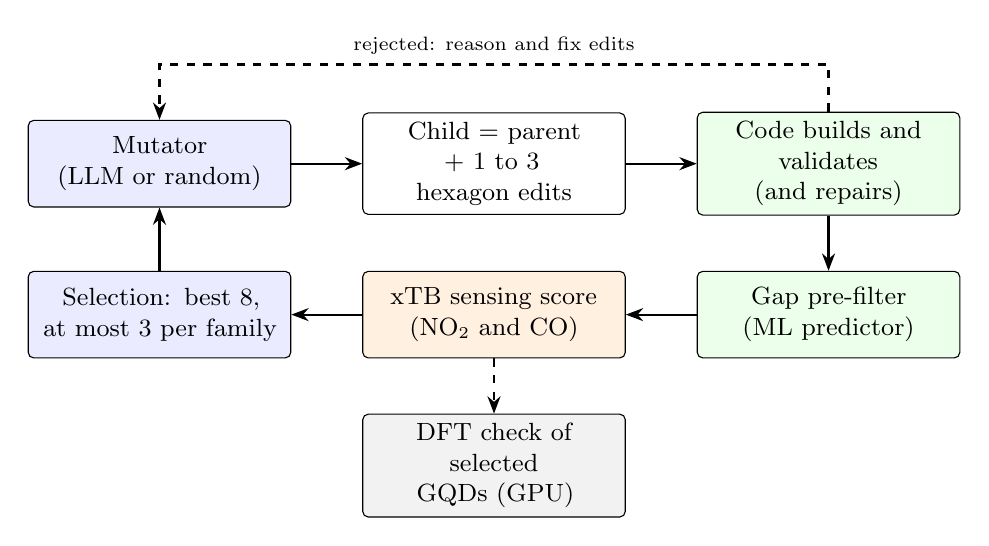
\begin{tikzpicture}[node distance=7mm and 9mm,
      box/.style={draw, rounded corners=2pt, align=center, font=\small, minimum height=11mm,
                  text width=31mm, fill=#1}, box/.default=white,
      arr/.style={-{Stealth[length=2.2mm]}, thick}]
    \node[box=blue!8] (mut) {Mutator\\(LLM or random)};
    \node[box, right=of mut] (edit) {Child = parent\\+ 1 to 3 hexagon edits};
    \node[box=green!8, right=of edit] (val) {Code builds and\\validates (and repairs)};
    \node[box=green!8, below=of val] (pre) {Gap pre-filter\\(ML predictor)};
    \node[box=orange!12, left=of pre] (xtb) {xTB sensing score\\(\ce{NO2} and CO)};
    \node[box=blue!8, left=of xtb] (sel) {Selection: best 8,\\at most 3 per family};
    \node[box=gray!10, below=of xtb] (dft) {DFT check of\\selected GQDs (GPU)};
    \draw[arr] (mut) -- (edit);
    \draw[arr] (edit) -- (val);
    \draw[arr] (val) -- (pre);
    \draw[arr] (pre) -- (xtb);
    \draw[arr] (xtb) -- (sel);
    \draw[arr] (sel) -- (mut);
    \draw[arr, dashed] (val.north) -- ++(0,6mm) -| node[pos=0.25, above, font=\scriptsize]
      {rejected: reason and fix edits} (mut.north);
    \draw[arr, dashed] (xtb) -- (dft);
  \end{tikzpicture}
  \caption{One generation of the evolutionary loop. The mutator proposes children as edits of
           the current best GQDs. Code turns each child into a molecule, checks it, and sends
           rejections back with the reason. A free ML prediction of the gap removes children
           outside a useful range, and GFN2-xTB scores the rest. The best GQDs scored so far
           become the next parents. Every proposal is logged, and selected GQDs are checked
           with DFT outside the loop.}
  \label{fig:pipeline}
\end{figure}

% ==========================================================================================
\section{The agent and its validation chain}
\label{sec:agent}

The project started as an agent built with LangGraph \cite{langgraph}, a library that describes an
LLM application as a graph of nodes that share a state. Before the agent, two small LangGraph
examples and a three-node graph that only read candidates from a table were written to learn the
library. The agent itself (\code{studio/agent.py}) is shown in \cref{fig:agent}.

The first node checks that the required software is present: the Python packages RDKit
\cite{rdkit}, NumPy, SciPy, PySCF \cite{sun2018pyscf} and geomeTRIC, and the \code{xtb} program. If
something is missing, the agent stops and says what is missing. Otherwise control passes to the
assistant node, where the LLM reads the conversation and either answers or calls a tool. The LLM is
GPT-5.4, accessed through an Azure OpenAI deployment (API version 2024-02-01) with LangChain
\cite{langchain}. Only one tool call is allowed per turn, because the validation nodes check one
structure at a time.

The agent has two tools. The first, \code{generate\_gqd}, returns a random SMILES string from a
pilot table of the existing dataset. It stood in for a structure generator while the graph was
being built. The second, \code{build\_gqd\_from\_hexagons}, lets the LLM design a GQD itself by
writing hexagon positions (\cref{sec:hex}).

Every structure that a tool returns passes through five checks in a fixed order:
\begin{enumerate}
  \item \emph{Molecular graph.} RDKit must parse and sanitise the SMILES, and the molecule must be
        one connected piece. Errors from the hexagon tool, such as an open-shell design, are
        reported at this step.
  \item \emph{Uniqueness.} The InChIKey must not already be among the saved structures.
  \item \emph{Ring count.} The molecule must have 20 to 40 six-membered rings.
  \item \emph{Hybridisation.} At least 95\% of the heavy atoms must be \(sp^2\).
  \item \emph{Synthetic accessibility.} The SA score \cite{ertl2009sascore} must be 8.0 or lower.
\end{enumerate}
These thresholds are the ones used to generate the original dataset. A structure that passes all
five is saved to a table together with a \code{.mol} file. A structure that fails goes back to the
LLM with the name of the failed step and the reason. The system prompt asks the LLM to fix its own
rejected designs and to give up after three rejections for the same request.

\begin{figure}[ht]
  \centering
  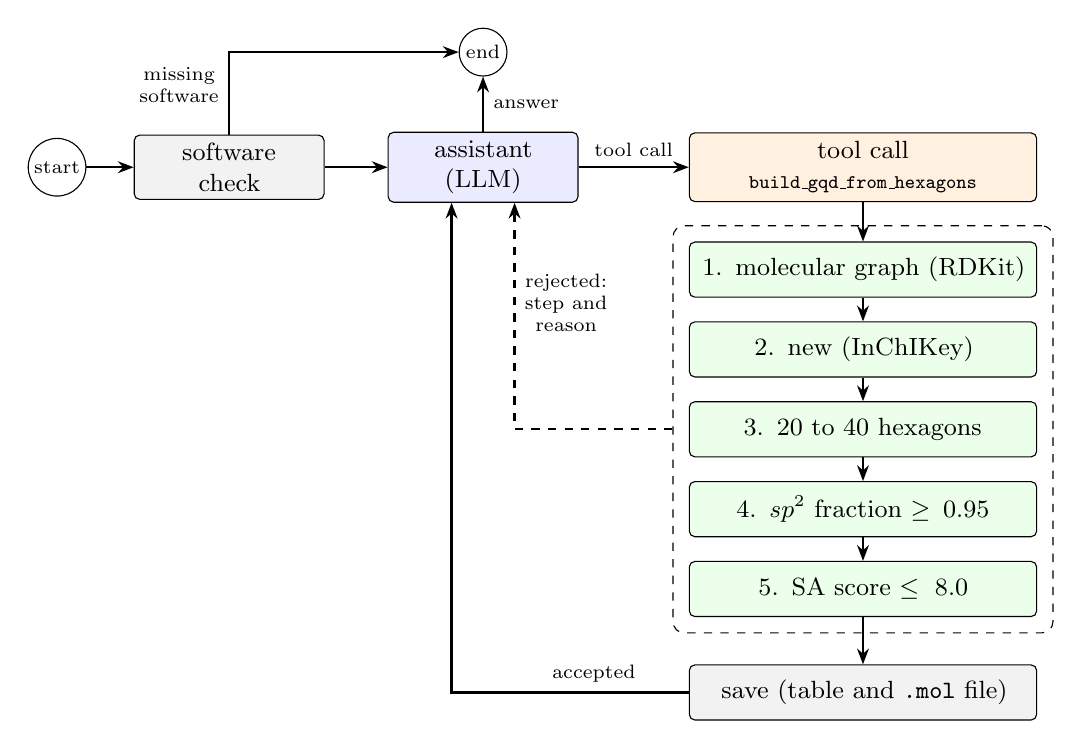
\begin{tikzpicture}[font=\small, node distance=8mm,
      st/.style={draw, rounded corners=2pt, align=center, minimum height=7mm, text width=#1,
                 inner sep=3pt},
      arr/.style={-{Stealth[length=2mm]}, thick},
      lab/.style={font=\scriptsize, align=center}]
    \node[draw, circle, inner sep=1.5pt, font=\scriptsize] (start) {start};
    \node[st=22mm, fill=gray!10, right=6mm of start] (sw) {software\\check};
    \node[st=22mm, fill=blue!8, right=of sw] (llm) {assistant\\(LLM)};
    \node[st=42mm, fill=orange!12, right=14mm of llm] (tools)
      {tool call\\{\scriptsize\code{build\_gqd\_from\_hexagons}}};
    \node[st=42mm, fill=green!8, below=5mm of tools] (c1) {1. molecular graph (RDKit)};
    \node[st=42mm, fill=green!8, below=3mm of c1] (c2) {2. new (InChIKey)};
    \node[st=42mm, fill=green!8, below=3mm of c2] (c3) {3. 20 to 40 hexagons};
    \node[st=42mm, fill=green!8, below=3mm of c3] (c4) {4. \(sp^2\) fraction \(\geq 0.95\)};
    \node[st=42mm, fill=green!8, below=3mm of c4] (c5) {5. SA score \(\leq 8.0\)};
    \node[st=42mm, fill=gray!10, below=6mm of c5] (save) {save (table and \code{.mol} file)};
    \begin{scope}[on background layer]
      \node[draw, dashed, rounded corners, fit=(c1)(c5), inner sep=2mm] (checks) {};
    \end{scope}
    \node[draw, circle, inner sep=1.5pt, font=\scriptsize, above=7mm of llm] (end) {end};
    \draw[arr] (start) -- (sw);
    \draw[arr] (sw) -- (llm);
    \draw[arr] (llm) -- node[lab, above] {tool call} (tools);
    \draw[arr] (tools) -- (c1);
    \draw[arr] (c1) -- (c2);
    \draw[arr] (c2) -- (c3);
    \draw[arr] (c3) -- (c4);
    \draw[arr] (c4) -- (c5);
    \draw[arr] (c5) -- (save);
    \draw[arr] (llm) -- node[lab, right] {answer} (end);
    \draw[arr] (sw.north) |- node[lab, pos=0.3, left] {missing\\software} (end.west);
    \draw[arr, dashed] (checks.west) -| node[lab, pos=0.78, right] {rejected:\\step and\\reason}
      ([xshift=4mm]llm.south);
    \draw[arr] (save.west) -| node[lab, pos=0.2, above] {accepted} ([xshift=-4mm]llm.south);
  \end{tikzpicture}
  \caption{The agent as a LangGraph state graph. The LLM proposes, and code decides: every
           structure passes the five checks in order, and a failure returns the step and the
           reason to the LLM.}
  \label{fig:agent}
\end{figure}

The agent established the rule that the rest of the work follows: the LLM may propose anything,
but only code decides whether a structure is accepted.

% ==========================================================================================
\section{Hexagon representation of GQDs}
\label{sec:hex}

\subsection{Coordinates}

A GQD is a set of fused hexagons on a honeycomb lattice, so it can be written as the list of
hexagons it occupies (\cref{fig:hexgrid}a). We use axial coordinates \((q,r)\). The six neighbours
of hexagon \((q,r)\) are \((q\pm1,r)\), \((q,r\pm1)\), \((q+1,r-1)\) and \((q-1,r+1)\). Benzene is
\([(0,0)]\), naphthalene is \([(0,0),(1,0)]\), and coronene is \((0,0)\) with its six neighbours.
In this form the number of rings is the length of the list, two hexagons are fused when they are
neighbours, and an edit to the shape is the addition or removal of one entry. The coordinate
convention and the rules for corners are the same as in the generator that produced the original
dataset.

\begin{figure}[ht]
  \centering
  \begin{subfigure}[b]{0.34\textwidth}
    \centering
    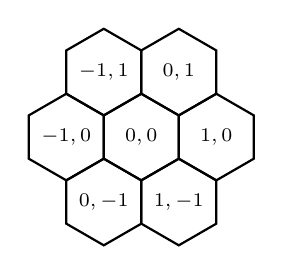
\begin{tikzpicture}[x=5.5mm, y=5.5mm]
      \foreach \qq/\rr in {0/0, 1/0, -1/0, 0/1, 0/-1, 1/-1, -1/1} {
        \begin{scope}[shift={({sqrt(3)*(\qq+0.5*(\rr))}, {1.5*(\rr)})}]
          \draw[thick] (90:1) -- (30:1) -- (-30:1) -- (-90:1) -- (-150:1) -- (150:1) -- cycle;
          \node[font=\scriptsize] at (0,0) {\(\qq,\rr\)};
        \end{scope}
      }
    \end{tikzpicture}
    \caption{Coronene, with \((q,r)\) of each hexagon.}
  \end{subfigure}\hfill
  \begin{subfigure}[b]{0.30\textwidth}
    \centering
    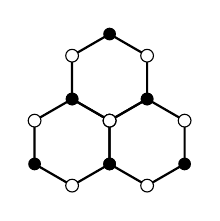
\begin{tikzpicture}[x=5.5mm, y=5.5mm]
      \foreach \qq/\rr in {0/0, 1/0, 0/1} {
        \begin{scope}[shift={({sqrt(3)*(\qq+0.5*(\rr))}, {1.5*(\rr)})}]
          \draw[thick] (90:1) -- (30:1) -- (-30:1) -- (-90:1) -- (-150:1) -- (150:1) -- cycle;
        \end{scope}
      }
      \foreach \qq/\rr in {0/0, 1/0, 0/1} {
        \begin{scope}[shift={({sqrt(3)*(\qq+0.5*(\rr))}, {1.5*(\rr)})}]
          \foreach \a in {90, 210, 330} \fill (\a:1) circle (2.3pt);
          \foreach \a in {30, 150, 270} \filldraw[fill=white, draw=black] (\a:1) circle (2.3pt);
        \end{scope}
      }
    \end{tikzpicture}
    \caption{Phenalenyl: 7 white and 6 black atoms. Open-shell.}
  \end{subfigure}\hfill
  \begin{subfigure}[b]{0.30\textwidth}
    \centering
    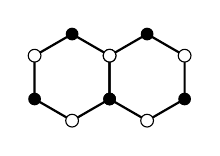
\begin{tikzpicture}[x=5.5mm, y=5.5mm]
      \foreach \qq/\rr in {0/0, 1/0} {
        \begin{scope}[shift={({sqrt(3)*(\qq+0.5*(\rr))}, {1.5*(\rr)})}]
          \draw[thick] (90:1) -- (30:1) -- (-30:1) -- (-90:1) -- (-150:1) -- (150:1) -- cycle;
        \end{scope}
      }
      \foreach \qq/\rr in {0/0, 1/0} {
        \begin{scope}[shift={({sqrt(3)*(\qq+0.5*(\rr))}, {1.5*(\rr)})}]
          \foreach \a in {90, 210, 330} \fill (\a:1) circle (2.3pt);
          \foreach \a in {30, 150, 270} \filldraw[fill=white, draw=black] (\a:1) circle (2.3pt);
        \end{scope}
      }
    \end{tikzpicture}
    \caption{Naphthalene: 5 white and 5 black atoms. Closed-shell.}
  \end{subfigure}
  \caption{The hexagon representation. (a) Axial coordinates. (b, c) The carbon atoms split into
           two sublattices (black and white), and every bond joins a black atom to a white one. A
           Kekul\'e structure needs equal numbers of the two, so the three-ring triangle in (b)
           must be a radical, while (c) is closed-shell.}
  \label{fig:hexgrid}
\end{figure}

\subsection{From hexagons to a molecule}

\Cref{alg:hex2mol} converts a hexagon list into an RDKit molecule. Each hexagon has six corners,
and a corner is named by the three grid positions that meet at it, so a corner shared by fused
hexagons becomes a single carbon atom. Each hexagon edge becomes a carbon-carbon bond, and each
carbon with only two carbon neighbours receives one hydrogen.

The double bonds are chosen by the code rather than by RDKit. A Kekul\'e structure is a perfect
matching of the carbon graph, and because the graph is bipartite, the augmenting-path method of
Kuhn \cite{kuhn1955hungarian} finds one or proves that none exists. We do this ourselves because
RDKit's kekulisation failed for some large GQDs depending on the order of the atoms: the same
structure passed or failed when its hexagons were listed in a different order. If no perfect
matching exists, the design is open-shell and is rejected. After sanitisation, the SMILES string
is written and read back. RDKit cannot re-read the SMILES of some valid closed-shell shapes, and
because every later step reads SMILES with RDKit, these shapes are rejected too
(\cref{sec:res-hex}).

The reverse function, \code{mol\_to\_hex}, places the first six-membered ring at \((0,0)\) and
walks across shared bonds: a ring that shares edge \(k\) of a placed hexagon must sit at the
neighbouring grid position for that edge. It returns the hexagon list or raises an error if the
rings do not fit on a flat honeycomb grid. A hexagon-sized hole has the same atoms and bonds as a
filled hexagon, so \code{mol\_to\_hex} returns such a structure with the hole filled.

\begin{algorithm}[ht]
  \caption{Hexagon list to molecule (\code{hex\_to\_mol})}
  \label{alg:hex2mol}
  \begin{algorithmic}[1]
    \Require list \(H\) of hexagon positions \((q,r)\); size range \([20,40]\)
    \State check that \(H\) has integer pairs, no duplicates and one connected piece
           \Comment{else reject}
    \For{each hexagon \(h \in H\) and each of its six corners}
      \State key \(\gets\) the three grid positions that meet at the corner
      \State create one carbon per distinct key; add a bond for each hexagon edge
    \EndFor
    \State \(M \gets\) perfect matching of the carbon graph (augmenting paths)
    \If{no perfect matching exists}
      \State \(N_A, N_B \gets\) sublattice counts; \(F \gets\) fix edits (\cref{alg:fixes})
      \State \textbf{reject} with ``open-shell, \(N_A\) vs \(N_B\)'' and the edits in \(F\)
    \EndIf
    \State make the bonds in \(M\) double and the rest single; add H to two-coordinate carbons
    \State sanitise with RDKit; write the SMILES and read it back \Comment{else reject}
    \State \Return the molecule
  \end{algorithmic}
\end{algorithm}

\subsection{Explaining an open-shell design}

An LLM cannot see the sublattice balance in a list of coordinates. When a design is open-shell, a
message such as ``no Kekul\'e form'' does not tell it what to change. The rejection message
therefore states the imbalance (for example ``33 vs 28, 5 unpaired atoms'') and lists concrete
edits that fix it (\cref{alg:fixes}). A corner belongs to sublattice A when the sum of \(q+r\) over
the three grid positions that meet there is 1 modulo 3, which makes the counts cheap to compute.
The code first tries every single edit, either adding a hexagon at an empty neighbouring position
or removing a hexagon whose removal keeps the shape connected, and keeps up to six edits that give
a closed-shell structure of allowed size. If no single edit works, a beam search (width 30) over
edit sequences of up to eight steps, ranked by the remaining imbalance \(|N_A-N_B|\), returns the
shortest sequence it finds. Every suggestion is checked with the exact matching test, and the
search takes about 0.1 to 0.5~s. The LLM still decides which edit to apply.

\begin{algorithm}[ht]
  \caption{Fix edits for an open-shell design (\code{open\_shell\_fixes})}
  \label{alg:fixes}
  \begin{algorithmic}[1]
    \Require open-shell hexagon set \(H\); size range \([20,40]\)
    \State \(E(H) \gets\) all single edits: add an empty neighbour, or remove a hexagon if the rest
           stays connected, within the size range
    \State \(F \gets \{e \in E(H) : H \oplus e \text{ has a Kekul\'e structure}\}\)
    \If{\(F \neq \emptyset\)}
      \State \Return up to six edits from \(F\)
    \EndIf
    \State frontier \(\gets \{(\,(),\,H)\}\)
    \For{depth \(= 1\) to 8}
      \For{each \((\text{path}, S)\) in frontier and each \(e \in E(S)\) not seen before}
        \If{\(S \oplus e\) has a Kekul\'e structure}
          \State \Return path \(+\,e\)
        \EndIf
      \EndFor
      \State frontier \(\gets\) the 30 new shapes with the smallest \(|N_A - N_B|\)
    \EndFor
    \State \Return no fix found
  \end{algorithmic}
\end{algorithm}

\subsection{The closed-shell rule in the prompt}
\label{sec:rule-prompt}

The second aid is a paragraph in the system prompt (\cref{app:prompts}). It explains that the
carbon atoms form two alternating sets that must be equal in number, names the shapes that usually
break this rule (triangles, L-shaped corners and long zigzag edges), and gives a simple way to
satisfy it: make the shape point-symmetric, so that for every \([q,r]\) the list also contains
\([a-q,b-r]\) for a fixed centre \((a/2,b/2)\). The centre of such an inversion is either a hexagon
centre or the midpoint of a shared bond, and in both cases the inversion maps every atom of one
sublattice onto an atom of the other, so the two counts are equal. Equal counts do not guarantee a
Kekul\'e structure, but in practice they remove most failures (\cref{sec:res-e1}).

\subsection{The dataset in hexagon form}

The existing dataset contains 91{,}174 GQDs with 20 to 40 hexagons, generated earlier in the
project by growing random hexagon clusters, given as SMILES. Each structure was converted to a
hexagon list with \code{mol\_to\_hex}, converted back with \code{hex\_to\_mol}, and kept only if
the canonical SMILES matched. Where available, xTB values of the HOMO, LUMO and gap were attached;
14{,}674 structures have them (4{,}600 from a first xTB batch and 10{,}074 from a second).

% ==========================================================================================
\section{Fast gap predictor}
\label{sec:predictor}

An xTB calculation takes minutes, while a prediction from a trained model takes milliseconds. The
predictor estimates the GFN2-xTB HOMO-LUMO gap of a GQD from its hexagon list or SMILES, together
with an uncertainty \(\sigma\). In the loop it is a free filter that removes children whose
gap is outside a useful range.

\paragraph{Data.} The 14{,}674 xTB-labelled GQDs were split 80/10/10 into training, validation and
test sets, stratified by gap. The 1{,}468 test structures were used only for the final report.

\paragraph{Baseline and features.} The H\"uckel gap, computed from the eigenvalues of the carbon
adjacency matrix, correlates with the xTB gap at \(r = 0.984\). A linear fit,
\(\Delta_{\mathrm{xTB}} \approx 2.5477\,\Delta_{\mathrm{H}} + 0.0527\)~eV with \(\Delta_{\mathrm{H}}\)
in units of \(|\beta|\), is the baseline, and the learned models predict only the residual. They
use 49 physics-based features: the H\"uckel spectrum near the gap (orbital energies, neighbouring
gaps, near-zero levels, orbital localisation and edge weight of the frontier orbitals), the
number of Kekul\'e structures and the Clar number, edge hydrogen types, perimeter features (bays,
coves, fjords), holes, and size and shape descriptors. A 2{,}048-bit Morgan fingerprint alone
reached only \(R^2 = 0.36\), so the physics features carry most of the signal.

\paragraph{Models.} LightGBM and XGBoost \cite{ke2017lightgbm,chen2016xgboost} were tuned with
Optuna \cite{akiba2019optuna} (100 trials each). A graph neural network in the style of GIN
\cite{xu2019gin} uses one node per carbon, with node features for edge position, ring membership,
hole contact and frontier-orbital coefficients, and receives the 49 features as global inputs.
Each model type was trained in five-fold cross-validation, and the fold models are averaged at
prediction time. Out-of-fold predictions set the ensemble weights (0.85 GNN and 0.15 XGBoost).

\paragraph{Uncertainty.} A LightGBM error model predicts the expected absolute error from the
features and from the disagreement between the models. It is scaled by 1.54 so that
\(\pm1.96\sigma\) covers 95\% of the out-of-fold errors. Inputs with fewer than 20 or more than
40 hexagons are refused, because the model is not valid there.

% ==========================================================================================
\section{\NOtwo{} sensing score}
\label{sec:score}

\subsection{Requirements}

A good \ce{NO2} sensing material has to meet three requirements. It must \emph{respond}: \ce{NO2}
should take electrons from the GQD, which changes the conductance of the layer, and more charge
means a larger signal. It must \emph{recover}: \ce{NO2} should not bind so strongly that it never
leaves. And it must be \emph{selective}: \ce{NO2} should bind more strongly than the other gases in
air, here water, ammonia and carbon monoxide. The function \code{evaluate\_gqd}
(\cref{alg:evaluate}) turns these requirements into numbers that GFN2-xTB can compute for any
hexagon list.

\subsection{Geometry and calculations}

The starting geometry of the GQD is built from the hexagon grid with \ce{C-C} bonds of 1.42~\AA{} and
\ce{C-H} bonds of 1.09~\AA{}. A small random out-of-plane displacement is added to every atom,
drawn from a normal distribution with a standard deviation of 0.05~\AA. The random generator is
seeded from the hexagon list, so the same GQD always starts from the same geometry. Most
GQDs in the dataset have crowded edges (coves or fjords) and are twisted at their minimum, and a
perfectly flat start gives the optimiser no force out of the plane; \cref{sec:res-flat} shows what
went wrong without the displacement. The GQD is then optimised with GFN2-xTB.

Two adsorption sites are probed: the hexagon closest to the centre of the GQD, and the most exposed
edge hexagon, defined as the hexagon with the fewest neighbours (ties broken by distance from the
centre). Each gas is placed above the centre of the site hexagon with its lowest atom 3.1~\AA{}
above the GQD plane. \ce{NO2} is placed in two orientations, with nitrogen down and with oxygen
down. \ce{H2O}, \ce{NH3}, CO and \ce{O2} use one orientation each. This gives 12 complexes, which
are optimised with GFN2-xTB in parallel. \ce{NO2} is a doublet and \ce{O2} a triplet, so these
complexes are computed with one and two unpaired electrons.

\subsection{Descriptors}

For each complex, the adsorption energy is
\begin{equation}
  \Eads = E(\text{GQD}+\text{gas}) - E(\text{GQD}) - E(\text{gas}),
  \label{eq:eads}
\end{equation}
where all three energies are from optimised structures. For each gas, the site and orientation
with the most negative \(\Eads\) are kept. From the \ce{NO2} complex we record the charge on the
\ce{NO2} atoms (the sum of the xTB atomic partial charges) and the shortest distance between the
gas and the GQD. A contact shorter than 1.9~\AA{} means that a covalent bond has formed, and the
\ce{NO2} is called chemisorbed. The recovery time is estimated as
\begin{equation}
  \tau = \nu^{-1}\exp\!\left(-\Eads/k_BT\right), \qquad \nu = 10^{12}~\text{s}^{-1},\; T = 298.15~\text{K}.
  \label{eq:tau}
\end{equation}

\subsection{Score}

The score multiplies a response term by two factors between 0 and 1:
\begin{align}
  S &= q_{\ce{NO2}} \times R \times \Sigma, \label{eq:score}\\
  R &= \operatorname{clip}\!\left(\frac{E_{\ce{NO2}} - E_{\mathrm{hard}}}{E_{\mathrm{soft}} - E_{\mathrm{hard}}},\,0,\,1\right),
      \qquad E_{\mathrm{soft}} = -0.6~\text{eV},\; E_{\mathrm{hard}} = -1.0~\text{eV}, \label{eq:rev}\\
  \Sigma &= \operatorname{clip}\!\left(\frac{\min_{g} E_g - E_{\ce{NO2}}}{0.10~\text{eV}},\,0,\,1\right),
      \qquad g \in \{\ce{H2O}, \ce{NH3}, \ce{CO}\}. \label{eq:sel}
\end{align}
Here \(q_{\ce{NO2}}\) is the number of electrons that move to \ce{NO2} (in units of \(e\)), and
\(E_{\ce{NO2}}\) and \(E_g\) are the strongest adsorption energies of \ce{NO2} and of each
interfering gas. The reversibility factor \(R\) is 1 when \ce{NO2} binds no more strongly than
\(-0.6\)~eV and falls linearly to 0 at \(-1.0\)~eV. By \cref{eq:tau}, recovery takes about 0.3~ms
at 0.5~eV, 7~s at 0.76~eV, 27~min at 0.9~eV and 22~h at 1.0~eV. The window is set somewhat lower
than a pure recovery argument would suggest because GFN2-xTB overbinds chemisorbed \ce{NO2} by 0.1
to 0.55~eV compared with DFT (\cref{sec:res-dft-small}). The selectivity factor \(\Sigma\) is 1
when \ce{NO2} binds at least 0.10~eV more strongly than the strongest interfering gas. \ce{O2} is
computed but not used in the score, because xTB describes it wrongly (\cref{sec:res-dft-small}).
The score has units of \(e\), and higher is better.

\begin{algorithm}[ht]
  \caption{\ce{NO2} sensing evaluation of one GQD (\code{evaluate\_gqd})}
  \label{alg:evaluate}
  \begin{algorithmic}[1]
    \Require hexagon list \(H\); gases \(G\) (all five, or \ce{NO2} and CO inside the loop)
    \State build a 3D geometry from \(H\) (\ce{C-C} 1.42~\AA, \ce{C-H} 1.09~\AA, small out-of-plane noise)
    \State optimise the GQD with GFN2-xTB \(\to E_{\mathrm{GQD}}\), gap
    \State sites \(\gets\) \{central hexagon, most exposed edge hexagon\}
    \ForAll{gas \(g \in G\), orientation of \(g\), site \(s\)} \Comment{in parallel}
      \State place \(g\) with its lowest atom 3.1~\AA{} above the centre of \(s\)
      \State optimise the complex with GFN2-xTB \(\to E\), atomic charges, shortest contact
      \State \(\Eads \gets E - E_{\mathrm{GQD}} - E_g\)
    \EndFor
    \State for each gas keep the site and orientation with the lowest \(\Eads\)
    \State compute \(q_{\ce{NO2}}\), chemisorption flag, \(\tau\), \(R\), \(\Sigma\) and \(S\)
           (\cref{eq:tau,eq:score,eq:rev,eq:sel})
    \State \Return all descriptors and \(S\)
  \end{algorithmic}
\end{algorithm}

\subsection{Cheaper scoring inside the loop}

A full evaluation needs 12 xTB optimisations and takes about 65~s per GQD (15 to 130~s) with
eight jobs in parallel on the laptop. Inside the evolutionary loop only \ce{NO2} and CO are
computed, which needs 6 optimisations. This does not change the score: on all 50 calibration GQDs,
CO was the strongest competing gas, and the score with \ce{NO2} and CO alone equalled the full
score (largest difference 0.000). \ce{H2O}, \ce{NH3} and \ce{O2} are computed again for the best
GQDs at the end of each run. xTB gains little from extra threads at this size, so five children are
scored side by side, each with six single-thread xTB jobs.

% ==========================================================================================
\section{Evolutionary loop}
\label{sec:loop}

\subsection{Population and edits}

The loop starts from the 50 GQDs used to calibrate the score (\cref{sec:e2}), which were scored
with all five gases. The population of each generation is the eight best GQDs scored so far
(\cref{alg:generation}). A child is made from one parent by one to three edits, where
\code{ADD [q, r]} adds a hexagon and \code{REMOVE [q, r]} removes one. Up to ten children per
generation are scored with xTB, and a run has ten generations. The two mutators produce edits in
different ways.

\paragraph{LLM mutator.} The LLM receives a system prompt (\cref{app:prompts}) with the hexagon
rules, the definition of the score, the edit format and the requirements a child must meet. The
user message lists the population, best first. For each parent it gives the identifier, score,
number of hexagons, xTB gap, \ce{NO2} adsorption energy, whether \ce{NO2} is physisorbed or
chemisorbed, the site where it binds best and that site's hexagon, the charge moved to \ce{NO2},
the margin over CO and the full hexagon list. It also lists every child of the previous generation
with its edits and its outcome: the score, or the reason it was rejected or skipped. The LLM
answers through a structured output schema: a list of children, each with a parent identifier, a
list of edits and a one-sentence reason. Rejected children are returned to the LLM with their
reasons, and it may propose more, for up to four rounds per generation. In each round it is asked
for 1.5 times the number of children still missing.

\paragraph{Random mutator.} The random mutator picks a parent from the population at random and
applies one random single-hexagon edit (with probability 2/3) or two (with probability 1/3).
The edits come from the same edit generator as the fix search, so they keep the shape connected
and within 20 to 40 hexagons. It may use up to 50 rounds per generation, because proposals are
free.

\subsection{Validation, repair and pre-filter}

Each child is built with \code{hex\_to\_mol} and checked with the ring-count, \(sp^2\) and SA
checks of the agent. Three further checks apply in the loop: the child must not have been made
before in the same run, must not be in the 91{,}174-structure dataset (compared by canonical
SMILES), and must have no holes. If a child fails only because it is open-shell, the code tries
the verified single-hexagon fixes of \cref{alg:fixes} and keeps the first one that passes every
check. The repair is logged, and the LLM sees it in the next generation (``code added \ldots'').
Valid children then go to the gap predictor, and a child is scored with xTB only if its predicted
gap lies between 0.20 and 1.60~eV. Below about 0.2~eV almost every calibration GQD chemisorbs
\ce{NO2}, and above 1.6~eV the charge moved to \ce{NO2} is smallest.

\subsection{Selection and final check}

The next population is the eight best GQDs scored so far whose xTB optimisations all converged.
To keep the population diverse, at most three of the eight may descend from the same starting
GQD; this lineage is called the family. At the end of a run the five best new GQDs are scored again
with all five gases.

\begin{algorithm}[ht]
  \caption{One generation of the evolutionary loop}
  \label{alg:generation}
  \begin{algorithmic}[1]
    \Require pool \(P\) of scored GQDs; mutator \(M\); dataset set \(K\); set \(U\) of structures made in this run
    \State population \(\gets\) best 8 converged GQDs in \(P\), at most 3 per family
    \State give \(M\) the population and the previous generation's results
    \State chosen \(\gets \emptyset\); feedback \(\gets\) none
    \For{round \(= 1\) to \(R_{\max}\) (4 for the LLM, 50 for random) \textbf{while} \(|\text{chosen}| < 10\)}
      \State proposals \(\gets M\)(number still needed, feedback)
      \ForAll{(parent, edits, reason) in proposals}
        \State child \(\gets\) parent with edits applied \Comment{reject if an edit is impossible}
        \State validate child; if it is only open-shell, try single-hexagon repairs
        \State reject if invalid, in \(U\), in \(K\) or with holes; else add child to \(U\)
      \EndFor
      \State predict gaps of the valid children; keep those in \([0.20, 1.60]\)~eV until 10 are chosen
      \State feedback \(\gets\) every rejection with its reason
    \EndFor
    \State score the chosen children with \code{evaluate\_gqd}(\ce{NO2}, CO), five at a time
    \State add scored children to \(P\); log every proposal with its outcome
  \end{algorithmic}
\end{algorithm}

\subsection{Logging}

Every proposal is written to a log, whether it was rejected, skipped or scored. The record contains
the generation, the goal, the parent's identifier, hexagons and score, the edits and the reason,
the child's hexagons, whether it was valid and why not, any repair, the predicted gap and its
uncertainty, and all xTB results (\cref{app:logging}). The LLM's prompts and replies are logged
separately. The logs make every run reproducible and resumable, and they are the training data for
the fine-tuning planned in \cref{sec:future}.

\subsection{Settings of the pilot and of the main runs}

The pilot runs (\cref{sec:res-pilot}) revealed problems that were fixed before the main
comparison. \Cref{tab:loop-versions} lists the differences. Both mutators received the same
changes.

\begin{table}[ht]
  \centering
  \caption{Loop settings in the pilot and in the main comparison (version 2).}
  \label{tab:loop-versions}
  \small
  \begin{tabularx}{\textwidth}{@{}Lll@{}}
    \toprule
    Setting & Pilot & Version 2 \\
    \midrule
    Repair of open-shell children by code & no & yes \\
    Family cap (parents from one starting GQD) & none & 3 \\
    Gap pre-filter window & 0.30 to 1.60~eV & 0.20 to 1.60~eV \\
    LLM proposal rounds per generation & 3 & 4 \\
    Population, children per generation, generations & 8, 10, 10 & 8, 10, 10 \\
    Seeds & 0 & 1, 2, 3 \\
    \bottomrule
  \end{tabularx}
\end{table}

% ==========================================================================================
\section{DFT checks}
\label{sec:dft-methods}

DFT is used to test where the xTB numbers can be trusted. All DFT calculations are single points
with \(\omega\)B97X-V \cite{mardirossian2014wb97xv} and the def2-SVP basis set \cite{weigend2005def2},
with VV10 nonlocal correlation \cite{vydrov2010vv10}, at the xTB-optimised geometries. Adsorption
energies follow \cref{eq:eads} without a counterpoise correction, so weak complexes are expected to
be overbound by about 0.1~eV \cite{boys1970counterpoise}. Charges are meta-L\"owdin populations
\cite{sun2014metalowdin}. Closed-shell systems use restricted Kohn-Sham (RKS), and complexes
with \ce{NO2} (doublet) or \ce{O2} (triplet) use unrestricted Kohn-Sham (UKS).

\paragraph{Small models on the laptop.} Tetracene, on which xTB chemisorbs \ce{NO2}, and coronene,
on which xTB physisorbs it, were computed with PySCF 2.14 on the laptop CPU. Full-size GQDs were too
slow there.

\paragraph{GPU benchmark.} Twelve GQDs were selected: ten calibration GQDs spread over the range of
scores, and the best GQD of each pilot run. Each was evaluated again with all five gases while
keeping every optimised geometry, which gives 156 complexes and GQDs plus 6 isolated gases, 162
single points in total. They are computed with GPU4PySCF 1.9.1 \cite{li2025gpu4pyscf} on one
NVIDIA A100 (80~GB), with integration grid level 3 (level 1 for VV10), an SCF convergence threshold
of \(10^{-8}\)~Hartree, and a second-order SCF fallback when the normal SCF does not converge.
Density fitting was tested and was slower than the exact integrals on the A100 for systems of this
size, so it is not used. The calculations run in three phases so that the most useful answers come
first: the GQDs with \ce{NO2} and CO, then \ce{O2}, then \ce{H2O} and \ce{NH3}. For each GQD the
descriptors and the score are recomputed from the DFT energies and charges with the same
formulas as for xTB.

\paragraph{Consistency check.} The benzene energy computed on the GPU, \(-232.014171\)~Hartree,
matches the laptop CPU value to all printed digits, at 4.5~s on the GPU against 61~s on the
laptop. A 134-atom GQD takes 99~s (RKS) and its \ce{NO2} complex 366~s (UKS).

% ==========================================================================================
\section{Computing environment}
\label{sec:compute}

Most of the work ran on a laptop: a MacBook Pro with an Apple M5 Pro processor (18 CPU cores) and
48~GB of memory, running macOS 27, Python 3.14, the conda-forge build of xTB 6.7.1, RDKit
2026.09.1, PySCF 2.14.0, LangGraph 1.2.20, langchain-openai 1.7.4, LightGBM 4.7.0, XGBoost 3.4.1,
PyTorch 2.15.0 and Optuna 5.0.0. The GPU calculations ran on a shared Linux server with two Intel
Xeon Silver 4309Y processors (16 cores in total), 503~GB of memory and two NVIDIA A100 80~GB GPUs
(CUDA 12.8), with Python 3.11, GPU4PySCF 1.9.1, PySCF 2.15.0 and CuPy 14.2. The same xTB evaluation
took about 6 times longer on the shared server CPU than on the laptop (394~s against about 65~s,
with an identical score), so all xTB work stayed on the laptop and the server was used for DFT.

% Chapter 4. Add a section for every new experiment and keep the status column of
% tab:experiments current (done / running / planned).
\chapter{Experimental design}
\label{ch:experiments}

This chapter defines the experiments that answer the research questions of \cref{sec:rq} and test
the hypotheses of \cref{sec:hypotheses}. \Cref{tab:experiments} gives an overview, and the
sections below give the design of each experiment: what is varied, what is held fixed, and what
is measured.

\begin{table}[ht]
  \centering
  \caption{Experiments, the questions they address and their status at the time of writing.}
  \label{tab:experiments}
  \small
  \begin{tabularx}{\textwidth}{@{}lLlll@{}}
    \toprule
    & Experiment & RQ & Hypothesis & Status \\
    \midrule
    E1 & LLM designs GQDs as hexagon lists: prompt \(\times\) feedback ablation & RQ1 & H1 & done \\
    E2 & Calibration of the sensing score on 50 dataset GQDs & RQ2, RQ4 & H2, H4 & done \\
    E3 & xTB against DFT on two small models (tetracene, coronene) & RQ2 & H2 & done \\
    E4 & xTB against DFT on 12 GQDs (GPU benchmark) & RQ2 & H2 & done \\
    E5a & Pilot: LLM against random mutation, one run each & RQ3, RQ4 & H3, H4 & done \\
    E5b & Main comparison: three runs per mutator, loop version 2 & RQ3, RQ4 & H3, H4 & done \\
    E6 & Baseline: random GQDs without evolution, same xTB budget & RQ3 & H3 & planned \\
    \bottomrule
  \end{tabularx}
\end{table}

% ==========================================================================================
\section{E1: LLM design with hexagon coordinates}
\label{sec:e1}

\paragraph{Question.} How often does the LLM produce a valid GQD when it writes hexagon positions,
and how much do the closed-shell rule in the prompt and the fix edits in the feedback help?

\paragraph{Requests.} Each request asks for one GQD with a target size drawn at random between 20
and 40 hexagons and one of eight shape descriptions: roughly round, elongated (a ribbon about three
hexagons wide), triangular, rectangular, irregular, mostly armchair edges, mostly zigzag edges, or
L-shaped. The same 80 requests (fixed random seed) are used in every condition. The requests go to
the same LLM deployment, tool and validation code as the agent. When a design fails, the rejection
message is returned and the LLM may retry up to two times.

\paragraph{Conditions.} A \(2 \times 2\) design varies the prompt and the feedback:
\begin{itemize}
  \item prompt: \emph{basic} (coordinates, neighbour rule and size only) or \emph{rule} (basic
        plus the closed-shell rule and the point-symmetry tip of \cref{sec:rule-prompt});
  \item feedback: \emph{plain} (``no Kekul\'e form'') or \emph{fixes} (the imbalance and the fix
        edits of \cref{alg:fixes}).
\end{itemize}
An earlier run of 50 requests with the basic prompt and plain feedback was used to find the main
cause of failure before the ablation was designed.

\paragraph{Measures.} Share of requests valid at the first attempt and after retries, mean number
of attempts, failed attempts by reason, number of distinct valid designs and the most repeated
design, novelty against the 91{,}174-structure dataset, share of point-symmetric designs, mean
deviation from the requested size, predicted gap range, and the number of designs with holes.

% ==========================================================================================
\section{E2: calibration of the sensing score}
\label{sec:e2}

\paragraph{Question.} How do the \ce{NO2} descriptors and the score vary across GQDs, and which
GQDs score best?

\paragraph{Sample.} Fifty GQDs were drawn from the 14{,}674 xTB-labelled structures, five from
each 0.2~eV bin of the dataset gap between 0 and 2.03~eV (random seed 0). They have 20 to 37
hexagons.

\paragraph{Procedure.} Each GQD was evaluated with all five gases (\cref{alg:evaluate}). As a
check of the geometry step, the gap of each optimised GQD was compared with the gap stored in the
dataset.

\paragraph{Measures.} Adsorption energy, charge transfer and chemisorption of \ce{NO2}; adsorption
energies of the interfering gases; selectivity margin; score; and their dependence on the gap. A
small classification study tested whether simple structural features predict chemisorption (area
under the ROC curve).

% ==========================================================================================
\section{E3: xTB against DFT on small models}
\label{sec:e3}

\paragraph{Question.} Where do GFN2-xTB adsorption energies and charges agree with DFT?

\paragraph{Systems.} Tetracene, on which xTB chemisorbs \ce{NO2}, and coronene, on which xTB
physisorbs it. These two cover both binding regimes and are small enough for DFT on the laptop.

\paragraph{Procedure.} The xTB-optimised complexes of all gases at both sites were recomputed with
DFT (\cref{sec:dft-methods}) at the same geometries.

\paragraph{Measures.} Adsorption energy and charge on the gas for every complex, from xTB and from
DFT.

% ==========================================================================================
\section{E4: xTB against DFT on twelve GQDs}
\label{sec:e4}

\paragraph{Question.} Does xTB rank full-size GQDs in the same order as DFT for the quantities
that enter the score, and do the best GQDs bind \ce{O2} in DFT?

\paragraph{Sample.} Ten calibration GQDs spread over the range of scores, and the best GQD of each
pilot run (\code{llm\_s0\_g10c004} and \code{random\_s0\_g02c004}).

\paragraph{Procedure.} 162 DFT single points on one A100 GPU, in three phases
(\cref{sec:dft-methods}).

\paragraph{Measures.} For each complex, the xTB and DFT adsorption energy and charge. For each GQD,
the descriptors and score from both methods. The main outcome is Spearman's rank correlation
\(\rho\) \cite{spearman1904} between xTB and DFT for \(E_{\ce{NO2}}\), \(q_{\ce{NO2}}\) and the
score. We fixed the decision rule before seeing the results:
\begin{itemize}
  \item \(\rho \geq 0.7\): xTB ranking is accepted, and the loop results stand as they are;
  \item \(0.4 \leq \rho < 0.7\): xTB is used for screening, and the top GQDs are re-ranked with
        DFT;
  \item \(\rho < 0.4\): the score must change, for example to a response term based on the HOMO
        energy or a correction learned from DFT.
\end{itemize}
The \ce{O2} adsorption energies give a first check of air stability.

% ==========================================================================================
\section{E5: LLM against random mutation}
\label{sec:e5}

\paragraph{Question.} With the same number of xTB evaluations, does the LLM mutator find better
GQDs than the random mutator?

\paragraph{Fixed across runs.} The starting pool (the 50 calibration GQDs; best score 0.322), the
validation and repair, the gap pre-filter, the number of generations (10) and of xTB-scored
children per generation (up to 10), the selection rule, and the final check. The xTB budget is
therefore at most 100 evaluations per run for both mutators.

\paragraph{Varied.} The mutator, and the random seed. In the pilot (E5a) each mutator ran once
with seed 0 and the first version of the loop. In the main comparison (E5b) each mutator runs three
times with seeds 1, 2 and 3 and version 2 of the loop (\cref{tab:loop-versions}). The seed fixes
all random choices of the loop. It does not fix the LLM, whose replies vary from call to call; for
the LLM runs the seed fixes only the loop around it.

\paragraph{Measures.} For each run: the number of proposals; the share that were valid; the share
that became valid only after repair by code; the number scored by xTB; the share of scored children
that beat their parent; the share that chemisorbed \ce{NO2}; the mean score of the scored children;
the best score; and the number of children above the best starting score. The curve of the best
score against the number of xTB evaluations shows sample efficiency. The number of LLM calls is
reported separately, because LLM calls are not part of the xTB budget.

\paragraph{Statistics.} For each mutator we report the mean and standard deviation over runs of
the best score and of the mean score. As a rough guide, a one-sided Mann-Whitney U test
\cite{mannwhitney1947} compares the scores of all scored children of the two mutators; children of
the same run are not independent, so this test overstates the evidence. With three runs per
mutator, a rank test on the per-run best scores cannot give a one-sided \(p\)-value below 0.05
(there are only 20 ways to split six runs into two groups of three). We therefore judge the main
comparison by the size of the differences and by whether they hold in every pair of runs, and not
by a significance threshold alone.

% ==========================================================================================
\section{E6: baseline without evolution (planned)}
\label{sec:e6}

The original plan compares three methods with the same xTB budget: random generation of new GQDs
without any evolution, evolution with random edits, and evolution with LLM edits. E5 covers the
last two. E6 will generate GQDs with the same random growth procedure that produced the dataset,
apply the same validation and pre-filter, and score about 100 of them with xTB. It shows how much
the evolutionary loop itself adds, independent of the mutator.
\pending{Run E6 after E5b finishes.}

% Chapter 5. Every number here comes from a result file in the repository; the source is
% given in a comment above each table. Replace \pending items as results arrive.
\chapter{Results}
\label{ch:results}

The results follow the order of the stages. \Cref{sec:res-hex,sec:res-predictor} report on the
tools that the experiments depend on, and the remaining sections report experiments E1 to E5
(\cref{tab:experiments}) and the features of the best GQDs.

% ==========================================================================================
\section{Hexagon conversion}
\label{sec:res-hex}
% Source: Stage1/README.md (run of 2026-11-10)

All 91{,}174 dataset structures converted to hexagon lists, and converting each list back gave the
original canonical SMILES in every case. The structures have 20 to 40 hexagons. Of these,
14{,}674 have xTB values, with gaps from 0.00 to 2.03~eV; another 1{,}326 xTB results could not be
used because their structures were missing from the SMILES table. In a separate test, 3{,}000
random hexagon clusters with 1 to 45 rings and 3{,}000 dataset structures were converted in both
directions. There were no mismatches, and the result did not depend on the order in which the
hexagons were listed.

One limitation of RDKit appeared in these tests. For about 10 to 14\% of closed-shell random shapes
with 20 to 40 rings, our code finds a valid Kekul\'e structure, but RDKit cannot read back the
SMILES it writes for the molecule (its kekulisation search gives up). Such shapes are rejected
because every later step depends on RDKit. None of the 91{,}174 dataset structures is affected,
and about 3\% of LLM designs were.

% ==========================================================================================
\section{Gap predictor}
\label{sec:res-predictor}
% Source: Stage2/README.md, Stage2/results/metrics.json

\Cref{tab:predictor} shows the errors on the 1{,}468 held-out test GQDs. The H\"uckel baseline
alone reaches a mean absolute error (MAE) of 0.042~eV. The boosted trees reduce this to 0.031~eV,
and the graph network to 0.022~eV. The ensemble used in the workflow has an MAE of 0.023~eV and
\(R^2 = 0.981\). For comparison, the earlier model of the parent project had an MAE of 0.386~eV on
the same structures.

\begin{table}[ht]
  \centering
  \caption{Gap predictor on the held-out test set (1{,}468 GQDs never used in training or
           tuning).}
  \label{tab:predictor}
  \small
  \begin{tabular}{@{}lrrr@{}}
    \toprule
    Model & MAE (eV) & RMSE (eV) & \(R^2\) \\
    \midrule
    H\"uckel gap, linear fit only & 0.0421 & 0.0721 & 0.966 \\
    LightGBM (5 folds) & 0.0308 & 0.0638 & 0.974 \\
    XGBoost (5 folds) & 0.0307 & 0.0635 & 0.974 \\
    GNN (5 folds) & 0.0216 & 0.0542 & 0.981 \\
    Ensemble, 0.85 GNN + 0.15 XGBoost (used) & 0.0226 & 0.0549 & 0.981 \\
    \quad GQDs without holes (\(n = 1{,}344\)) & 0.0181 & 0.0441 & 0.988 \\
    \quad GQDs with holes (\(n = 124\)) & 0.0712 & 0.1208 & 0.863 \\
    \bottomrule
  \end{tabular}
\end{table}

The uncertainty is well calibrated: 96.7\% of test GQDs fall within \(\pm1.96\sigma\), against a
target of 95\%. The mean \(\sigma\) is 0.029~eV for GQDs without holes and 0.114~eV for GQDs with
holes, so the model reports larger uncertainty where its errors are larger. The rank correlation
between \(\sigma\) and the actual absolute error is 0.33. Errors grow modestly outside the training
distribution. For test gaps outside the central 90\% of the training gaps, the LightGBM MAE is
0.049~eV (H\"uckel baseline 0.064~eV), and a LightGBM model trained on GQDs with at most 34 hexagons
has an MAE of 0.033~eV on GQDs with 35 or more. Prediction takes about 4.5~s for 200 GQDs, most of
it spent starting the GNN process, and the full training took 78 minutes on the laptop CPU.

Structures with holes are four times harder to predict, and they make up 8.5\% of the data. This
was one of the reasons the evolutionary loop rejects holes (\cref{sec:loop}).

% ==========================================================================================
\section{E1: the LLM designs GQDs as hexagon lists}
\label{sec:res-e1}
% Source: Stage2d/README.md, Stage2d/results/ablation.md

In the first run (50 requests, basic prompt, plain feedback), 46\% of requests gave a valid GQD at
the first attempt and 64\% after up to two retries. Of the 67 failed attempts, 66 were open-shell
designs. The LLM wrote connected, duplicate-free lists of the right size, but it could not tell
which shapes have unequal sublattices, and the message ``no Kekul\'e form'' did not tell it what to
change.

\Cref{tab:e1} shows the ablation. Each aid helps in a different way. The closed-shell rule in the
prompt raises the first-attempt pass rate from 34\% to 56\% (plain feedback) and 57\% (fix edits), because fewer designs are
open-shell to begin with. The fix edits make retries work: with the basic prompt they raise the
final pass rate from 52\% to 90\%. With both aids, 79 of 80 requests (99\%) ended in a valid GQD,
the mean number of attempts fell from 2.21 to 1.53, and open-shell attempts fell from 131 to 39.
Shapes that had almost always failed now succeeded: with both aids, L-shaped, triangular and
irregular requests went from 1, 3 and 0 valid designs out of 10 to 10 out of 10 each. Almost all
valid designs were new compared with the dataset, and none had holes.

\begin{table}[ht]
  \centering
  \caption{E1 ablation: 80 identical requests per condition, up to two retries. Prompt: basic or
           with the closed-shell rule. Feedback: plain or with fix edits.}
  \label{tab:e1}
  \small
  \begin{tabular}{@{}lrrrr@{}}
    \toprule
    & basic, plain & basic, fixes & rule, plain & rule, fixes \\
    \midrule
    Valid at first attempt & 34\% & 36\% & 56\% & 57\% \\
    Valid after \(\leq 2\) retries & 52\% & 90\% & 82\% & \textbf{99\%} \\
    Mean attempts per request & 2.21 & 1.83 & 1.66 & 1.53 \\
    Failed attempts: open-shell & 131 & 67 & 63 & 39 \\
    Failed attempts: other reasons & 4 & 7 & 4 & 4 \\
    Valid designs & 42 & 72 & 66 & 79 \\
    Distinct valid designs & 33 & 67 & 45 & 55 \\
    Most repeated design & \(\times 4\) & \(\times 2\) & \(\times 11\) & \(\times 9\) \\
    New compared with the dataset & 42/42 & 70/72 & 66/66 & 79/79 \\
    Point-symmetric & 45\% & 24\% & 58\% & 48\% \\
    Mean size error (hexagons) & 0.4 & 0.9 & 1.7 & 1.9 \\
    Predicted gap range (eV) & 0.05--1.42 & 0.02--1.27 & 0.07--1.40 & 0.01--1.51 \\
    \bottomrule
  \end{tabular}
\end{table}

The rule prompt has a cost. With it, the LLM often fell back on a standard symmetric shape: one
design appeared 11 times in 80 requests with plain feedback and 9 times with fix edits. The fix
edits alone kept the most variety (67 distinct designs out of 72 valid ones). Designs also drifted
from the requested size by about two hexagons when fixes or symmetry were applied, though they
always stayed within 20 to 40. In the agent, repeats are caught by the uniqueness check, and in
the evolutionary loop variety comes from editing different parents.

LLM results vary between runs. The basic-prompt, plain-feedback condition gave 46\% and 64\% in
the first run and 34\% and 52\% when repeated in the ablation. Conditions should therefore be
compared within the same run, as in \cref{tab:e1}.

% ==========================================================================================
\section{E2: the sensing score on 50 dataset GQDs}
\label{sec:res-e2}
% Source: Stage3a/README.md, Stage3a/results/summary.md, Stage3a/data/calibration.csv

\subsection{A geometry problem found and fixed}
\label{sec:res-flat}

The first calibration run started every GQD perfectly flat. Nearly all dataset GQDs have crowded
edges, coves or fjords, in 48 of the 50 sampled here, and their relaxed shape is twisted. A flat
start has no force out of the plane, so the optimiser kept these GQDs flat and strained. When a gas
was added, it broke the symmetry, the GQD twisted and released its strain, and the released energy
was counted as adsorption energy. In the worst case water appeared to bind by \(-6.3\)~eV. With
the small random out-of-plane displacement (\cref{sec:score}), 48 of the 50 GQDs relaxed to
structures more than 0.5~\AA{} out of plane, and the xTB gaps of our optimised GQDs agreed with the
dataset gaps with a mean absolute difference of 0.036~eV (\(r = 0.984\)). The flawed run is kept
in the repository for reference, and all results below come from the corrected run.

\subsection{Descriptors}

All 50 evaluations finished and every optimisation converged. \Cref{tab:calibration} groups the
results by gap, and \cref{fig:sensing-vs-gap} shows them for every GQD.

\begin{table}[ht]
  \centering
  \caption{E2: \ce{NO2} sensing descriptors of 50 dataset GQDs (10 per gap range; medians unless
           stated). Adsorption energies in eV, charge in \(e\).}
  \label{tab:calibration}
  \small
  \begin{tabular}{@{}lccccc@{}}
    \toprule
    Gap (eV) & \(E_{\ce{NO2}}\) & Chemisorbed & \(q_{\ce{NO2}}\) & \ce{H2O} / \ce{NH3} / CO & Score, median (max) \\
    \midrule
    0.0--0.4 & \(-1.15\) & 9/10 & 0.21 & \(-0.13\) / \(-0.14\) / \(-0.23\) & 0.00 (0.28) \\
    0.4--0.8 & \(-0.66\) & 7/10 & 0.21 & \(-0.14\) / \(-0.14\) / \(-0.24\) & 0.18 (0.32) \\
    0.8--1.2 & \(-0.38\) & 3/10 & 0.22 & \(-0.15\) / \(-0.16\) / \(-0.25\) & 0.22 (0.26) \\
    1.2--1.6 & \(-0.62\) & 6/10 & 0.22 & \(-0.15\) / \(-0.15\) / \(-0.25\) & 0.12 (0.25) \\
    1.6--2.1 & \(-0.34\) & 4/10 & 0.19 & \(-0.15\) / \(-0.16\) / \(-0.23\) & 0.15 (0.20) \\
    \bottomrule
  \end{tabular}
\end{table}

\begin{figure}[ht]
  \centering
  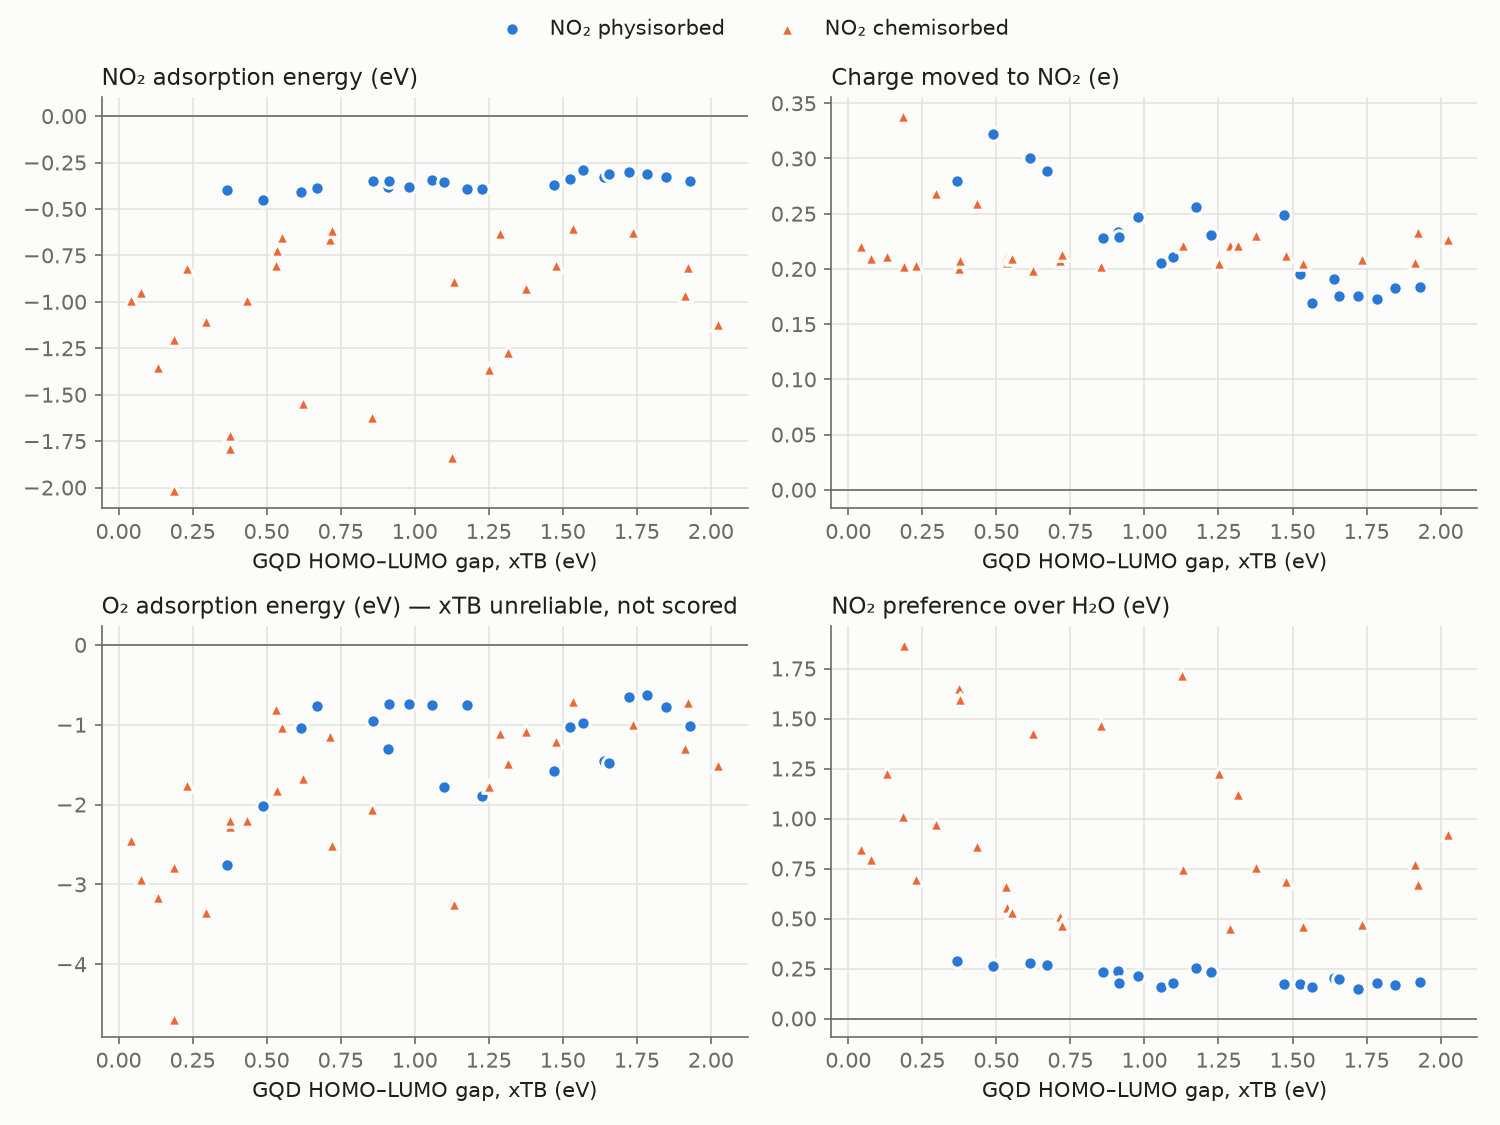
\includegraphics[width=\textwidth]{stage3a_sensing_vs_gap.png}
  \caption{E2: descriptors of the 50 calibration GQDs against their xTB gap. Circles: \ce{NO2}
           physisorbed; triangles: \ce{NO2} chemisorbed (contact shorter than 1.9~\AA). Top left:
           \ce{NO2} adsorption energy. Top right: charge moved to \ce{NO2}. Bottom left: \ce{O2}
           adsorption energy, which xTB describes wrongly and which is not scored. Bottom right:
           how much more strongly \ce{NO2} binds than \ce{H2O}.}
  \label{fig:sensing-vs-gap}
\end{figure}

\ce{NO2} binds in two distinct ways. In 21 of the 50 GQDs it physisorbs, at \(-0.29\) to
\(-0.45\)~eV, which corresponds to a recovery time well below one second. In the other 29 a
carbon-nitrogen bond forms, and xTB gives \(-0.6\) to \(-2.0\)~eV. Chemisorption is much more
common at small gaps (9 of 10 GQDs below 0.4~eV) but occurs at every gap, because it depends on the
local site rather than on the GQD as a whole. Simple structural features predicted it only weakly;
the best single predictors (many isolated edge \ce{C-H} groups, fewer Kekul\'e structures and a smaller
gap) reached an area under the ROC curve of at most 0.73.

For physisorbed \ce{NO2}, the charge moved to \ce{NO2} grows as the gap shrinks, from about
0.17~\(e\) at a gap of 1.9~eV to about 0.32~\(e\) at 0.5~eV. A smaller gap goes with a higher HOMO,
so the GQD gives up electrons more easily. Selectivity among the interfering gases was never the
limiting factor. CO was the strongest competitor in all 50 GQDs, but \ce{NO2} always bound more
strongly, by 0.1 to 0.2~eV in the physisorbed GQDs.

\subsection{Score}

Thirty-eight of the 50 GQDs scored above zero (\cref{fig:score-vs-gap}). The best scores, 0.28 to
0.32, all came from GQDs that physisorb \ce{NO2} and have a gap of about 0.35 to 0.7~eV. The three
best were \code{gqd\_18941} (score 0.32, gap 0.49~eV), \code{gqd\_23821} (0.30, 0.61~eV) and
\code{gqd\_90531} (0.29, 0.67~eV). This range is also where the trade-off is sharpest: 7 of the 10
dataset GQDs with gaps between 0.4 and 0.8~eV chemisorb \ce{NO2} and score low. Finding a GQD with a
small gap that still physisorbs \ce{NO2} is therefore the actual design problem, and it became the
goal of the evolutionary loop.

\begin{figure}[ht]
  \centering
  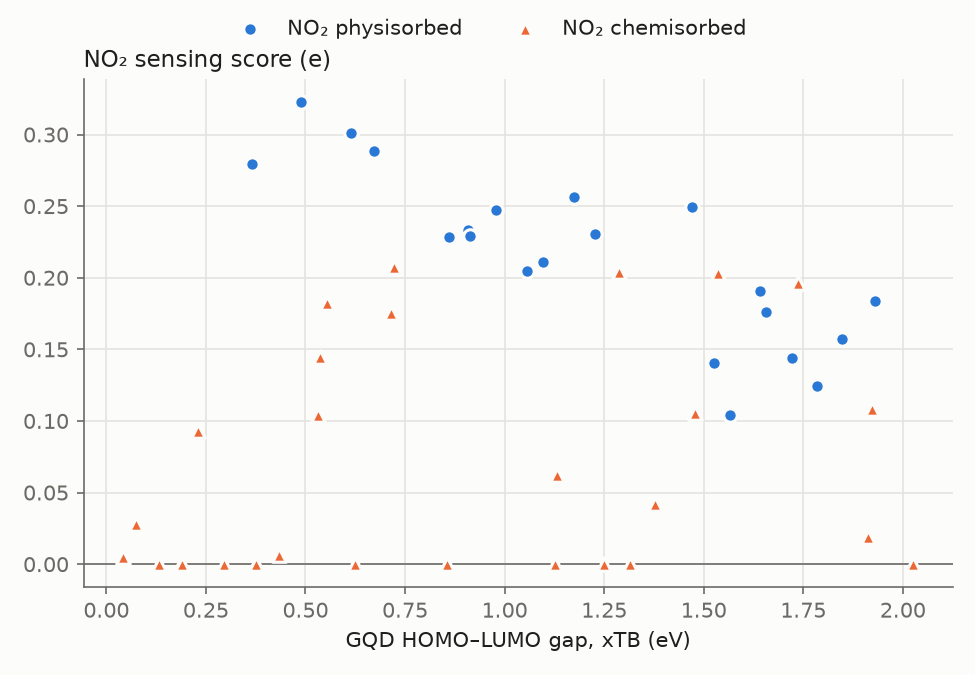
\includegraphics[width=0.8\textwidth]{stage3a_score_vs_gap.png}
  \caption{E2: \ce{NO2} sensing score of the 50 calibration GQDs against their xTB gap. The best
           scores come from physisorbing GQDs with gaps of about 0.35 to 0.7~eV. Chemisorbing GQDs
           (triangles) are penalised by the reversibility factor.}
  \label{fig:score-vs-gap}
\end{figure}

% ==========================================================================================
\section{E3: xTB against DFT on small models}
\label{sec:res-dft-small}
% Source: Stage3a/README.md, Stage3a/data/dft_check/

\Cref{tab:dft-tetracene,tab:dft-coronene} compare xTB and DFT at the same geometries.

\begin{table}[ht]
  \centering
  \caption{E3: tetracene, on which xTB chemisorbs \ce{NO2}. Energies in eV, charges on the gas in
           \(e\) (xTB charges; meta-L\"owdin for DFT).}
  \label{tab:dft-tetracene}
  \small
  \begin{tabular}{@{}lrrrrr@{}}
    \toprule
    Complex & Distance (\AA) & \(\Eads\) xTB & \(\Eads\) DFT & \(q\) xTB & \(q\) DFT \\
    \midrule
    \ce{NO2}, centre (chemisorbed) & 1.52 & \(-1.20\) & \(-0.76\) & 0.20 & 0.19 \\
    \ce{NO2}, edge (chemisorbed) & 1.53 & \(-0.74\) & \(-0.19\) & 0.19 & 0.19 \\
    \ce{NO2}, O down (chemisorbed) & 1.47 & \(-0.68\) & \(-0.59\) & 0.26 & 0.27 \\
    \ce{O2}, centre & 1.45 & \(-1.52\) & \(+0.53\) & 0.34 & 0.28 \\
    \ce{O2}, edge & 1.46 & \(-1.07\) & \(+1.10\) & 0.36 & 0.28 \\
    \ce{H2O} & 2.69 & \(-0.12\) & \(-0.24\) & 0.01 & 0.01 \\
    \bottomrule
  \end{tabular}
\end{table}

\begin{table}[ht]
  \centering
  \caption{E3: coronene, on which xTB physisorbs \ce{NO2}. Units as in \cref{tab:dft-tetracene}.}
  \label{tab:dft-coronene}
  \small
  \begin{tabular}{@{}lrrrrr@{}}
    \toprule
    Complex & Distance (\AA) & \(\Eads\) xTB & \(\Eads\) DFT & \(q\) xTB & \(q\) DFT \\
    \midrule
    \ce{NO2}, centre & 3.06 & \(-0.19\) & \(-0.20\) & 0.04 & 0.00 \\
    \ce{NO2}, edge & 2.55 & \(-0.24\) & \(-0.06\) & 0.13 & 0.04 \\
    \ce{NO2}, O down, centre & 2.87 & \(-0.18\) & \(-0.20\) & 0.09 & 0.00 \\
    \ce{NO2}, O down, edge & 2.75 & \(-0.18\) & \(-0.20\) & 0.09 & 0.00 \\
    \ce{O2}, edge & 2.62 & \(-0.51\) & \(+0.23\) & 0.30 & 0.03 \\
    \ce{O2}, centre & 2.59 & \(-0.47\) & \(+3.74\)\(^{a}\) & 0.30 & 0.36\(^{a}\) \\
    CO, centre / edge & 3.2 & \(-0.09\) / \(-0.07\) & \(-0.08\) / \(-0.06\) & 0.01 & 0.01 \\
    \ce{NH3}, centre / edge & 2.9 & \(-0.14\) / \(-0.13\) & \(-0.22\) / \(-0.19\) & 0.00 & 0.00 \\
    \ce{H2O}, centre / edge & 2.7 & \(-0.13\) / \(-0.12\) & \(-0.26\) / \(-0.24\) & 0.01 & 0.01 \\
    \bottomrule
    \multicolumn{6}{@{}l}{\footnotesize \(^{a}\) Probably converged to a wrong, charge-separated
      electronic state. \ce{O2} is unbound in DFT either way.}
  \end{tabular}
\end{table}

Four findings follow. First, for the closed-shell gases and for physisorbed \ce{NO2}, xTB
adsorption energies are close to DFT, mostly within 0.1~eV. The larger DFT binding of \ce{H2O}
(\(-0.24\) to \(-0.26\)~eV) is consistent with the overbinding expected from the small basis set
without counterpoise correction. Second, the \ce{NO2} chemisorption seen in xTB is real, since DFT
also binds the bonded complexes, but xTB overbinds them by 0.1 to 0.55~eV. Third, the charge moved
to \ce{NO2} agrees within about 0.01~\(e\) for chemisorbed \ce{NO2}, but for physisorbed \ce{NO2}
xTB overestimates it (0.04 to 0.13~\(e\) against 0.00 to 0.04~\(e\) on coronene). This is the
over-delocalisation expected from a DFT-like method \cite{cohen2008insights}. Across the 21
physisorbing calibration GQDs, the xTB charge still follows the GQD's HOMO energy closely
(\(r = 0.88\)), and a higher HOMO means a better electron donor, which is the physically expected
direction. The response term therefore ranks GQDs sensibly, but its absolute values for
physisorption are too large. Fourth, xTB binds \ce{O2} (\(-0.5\) to \(-1.5\)~eV), while DFT finds
it unbound in every case. \ce{O2} was therefore left out of the score, and the air stability of
the final candidates has to be checked with DFT.

% ==========================================================================================
\section{E5a: pilot comparison of LLM and random mutation}
\label{sec:res-pilot}
% Source: Stage3/README.md, Stage3/results/compare.md, Stage3/results/{llm_s0,random_s0}/

Both pilot runs started from the same population (best score 0.322) and took about 55 minutes
each on the laptop. \Cref{tab:pilot} summarises them and \cref{fig:pilot} shows their progress.

\begin{table}[ht]
  \centering
  \caption{E5a: pilot runs, 10 generations, one run per mutator (seed 0, loop version 1).}
  \label{tab:pilot}
  \small
  \begin{tabular}{@{}lrr@{}}
    \toprule
    & LLM & random \\
    \midrule
    Children proposed & 300 & 300 \\
    Valid (passed all checks) & 31\% & 54\% \\
    Scored by xTB & 80 & 100 \\
    Scored children that beat their parent & 11\% & 11\% \\
    Scored children with chemisorbed \ce{NO2} & 35\% & 47\% \\
    Mean score of scored children & 0.211 & 0.190 \\
    Best score & \textbf{0.340} & 0.331 \\
    Children above the best starting score (0.322) & 10 & 9 \\
    \bottomrule
  \end{tabular}
\end{table}

\begin{figure}[ht]
  \centering
  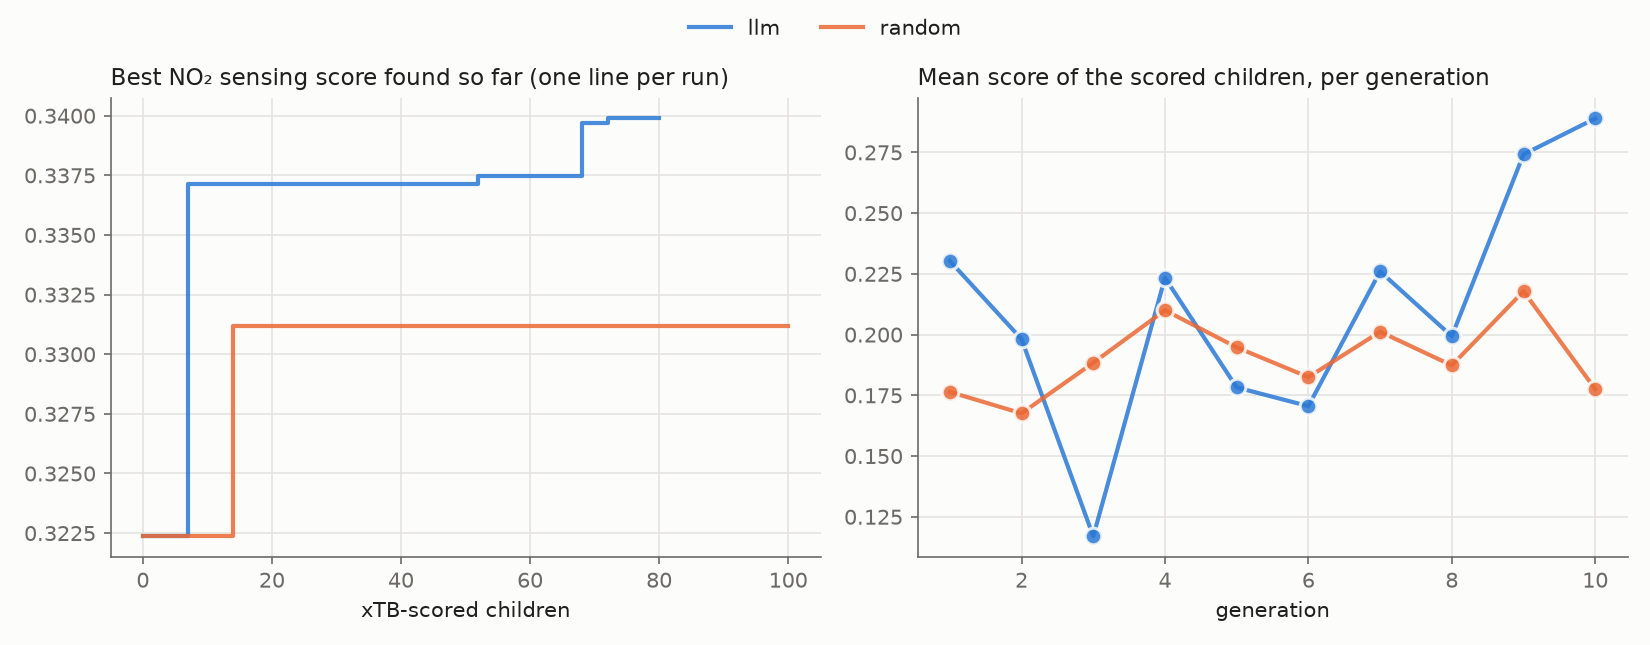
\includegraphics[width=\textwidth]{stage3_pilot_compare.png}
  \caption{E5a: pilot runs. Left: best score found so far against the number of xTB-scored
           children (the vertical axis is zoomed in). Right: mean score of the scored children in
           each generation.}
  \label{fig:pilot}
\end{figure}

The LLM run found the best GQD (0.340 against 0.331) with fewer xTB evaluations. It passed the best
starting score after 7 scored children, against 14 for the random run, and its children
chemisorbed \ce{NO2} less often. Its mean score per generation rose in the last two generations
(0.27 to 0.29, against 0.18 to 0.22 for random). With one run per mutator, however, the difference
in scores is not significant (one-sided Mann-Whitney \(p = 0.20\) on the scores of all scored
children), and the gain over the start, 0.018, is about the size of the noise from xTB and from
probing only two sites.

The ten best new GQDs (five per run) were scored again with all five gases. The loop score
matched the full score within 0.002 in every case, CO was always the strongest competing gas, and
\ce{NO2} bound more strongly than \ce{H2O} by at least 0.27~eV. \Cref{tab:pilot-best} lists the
best of them. All physisorb \ce{NO2}. The LLM's best GQDs have gaps of 0.29 to 0.33~eV, smaller
than any of the best calibration GQDs, while still physisorbing \ce{NO2}.

\begin{table}[ht]
  \centering
  \caption{E5a: best GQDs of the pilot runs after the full check with all gases. Margins are
           \(E_g - E_{\ce{NO2}}\) for CO and \ce{H2O}; positive means \ce{NO2} binds more strongly.}
  \label{tab:pilot-best}
  \small
  \begin{tabular}{@{}llrrrrrrr@{}}
    \toprule
    GQD & Run & Hexagons & Gap & \(E_{\ce{NO2}}\) & \(q_{\ce{NO2}}\) & CO margin & \ce{H2O} margin & Score \\
        &     &          & (eV) & (eV) & (\(e\)) & (eV) & (eV) & (\(e\)) \\
    \midrule
    g10c004 & LLM & 38 & 0.29 & \(-0.50\) & 0.34 & \(+0.25\) & \(+0.31\) & 0.341 \\
    g10c007 & LLM & 37 & 0.30 & \(-0.50\) & 0.34 & \(+0.25\) & \(+0.31\) & 0.340 \\
    g09c019 & LLM & 38 & 0.33 & \(-0.49\) & 0.34 & \(+0.25\) & \(+0.33\) & 0.340 \\
    g07c026 & LLM & 36 & 0.30 & \(-0.49\) & 0.34 & \(+0.24\) & \(+0.31\) & 0.338 \\
    g01c022 & LLM & 35 & 0.31 & \(-0.49\) & 0.34 & \(+0.25\) & \(+0.30\) & 0.337 \\
    g02c004 & random & 35 & 0.36 & \(-0.49\) & 0.33 & \(+0.24\) & \(+0.30\) & 0.331 \\
    g07c013 & random & 33 & 0.45 & \(-0.47\) & 0.33 & \(+0.22\) & \(+0.28\) & 0.331 \\
    \bottomrule
  \end{tabular}
\end{table}

The pilot also exposed three problems with the loop.
\begin{enumerate}
  \item \emph{Low validity of LLM children (31\%).} Of the 300 LLM proposals, 100 were
        open-shell, partly because the LLM often used two or three edits per child, while the
        random mutator mostly used one. Another 43 were duplicates, about 30 contained bookkeeping
        errors (adding a hexagon that was already there or removing one that was not), and 10 used
        four edits. As a result, 6 of the 10 LLM generations scored fewer than 10 children.
  \item \emph{Loss of diversity.} By generation 10, all eight LLM parents descended from one
        starting GQD (\code{gqd\_14650}). The random run kept two families.
  \item \emph{Gap floor.} The LLM's best GQDs sat at the lower edge of the 0.30~eV pre-filter, and
        about 10 LLM children were skipped for a predicted gap below 0.30~eV.
\end{enumerate}
These problems led to version 2 of the loop (\cref{tab:loop-versions}). Applied to the pilot's
proposals, the open-shell repair alone would have raised validity from 31\% to 50\% for the LLM
and from 54\% to 81\% for random mutation. In addition, xTB gave \ce{O2} adsorption energies of
\(-2.7\) to \(-3.4\)~eV for the best GQDs, which is consistent with the known \ce{O2} error of xTB
(\cref{sec:res-dft-small}) but means that air stability must be checked with DFT.

% ==========================================================================================
\section{E5b: main comparison of LLM and random mutation}
\label{sec:res-main}
% Source: Stage3/results/compare_v2.md and compare_v2.png, made by
%   Stage3/compare.py llm_v2_s1 llm_v2_s2 llm_v2_s3 random_v2_s1 random_v2_s2 random_v2_s3 --name v2
% from Stage3/results/{llm,random}_v2_s{1,2,3}/children.jsonl; LLM calls from llm_log.jsonl;
% full checks from final_check.csv. random_v2_s3 was interrupted after generation 5 and resumed
% with the same seed.

All six runs of loop version 2 finished. \Cref{tab:main} gives the result of each run,
\cref{tab:main-mutator} the mean and standard deviation over the three runs of each mutator, and
\cref{fig:main} the progress of each run.

\begin{table}[ht]
  \centering
  \caption{E5b: the six runs of loop version 2 (10 generations each, seeds 1 to 3). ``Repaired'' is
           the share of all proposals that became valid only after repair by code.}
  \label{tab:main}
  \small
  \begin{tabular}{@{}lrrrrrr@{}}
    \toprule
    & \multicolumn{3}{c}{LLM} & \multicolumn{3}{c}{random} \\
    \cmidrule(lr){2-4}\cmidrule(l){5-7}
    & s1 & s2 & s3 & s1 & s2 & s3 \\
    \midrule
    Children proposed & 207 & 255 & 191 & 300 & 300 & 300 \\
    Valid & 59\% & 45\% & 60\% & 84\% & 84\% & 79\% \\
    Repaired by code & 39\% & 28\% & 41\% & 33\% & 33\% & 32\% \\
    Scored by xTB & 99 & 100 & 100 & 100 & 100 & 100 \\
    Beat their parent & 13\% & 12\% & 7\% & 13\% & 9\% & 5\% \\
    \ce{NO2} chemisorbed & 49\% & 54\% & 51\% & 52\% & 65\% & 60\% \\
    Mean score of scored children & 0.194 & 0.172 & 0.191 & 0.178 & 0.157 & 0.154 \\
    Best score & 0.342 & 0.343 & 0.348 & \textbf{0.356} & 0.354 & 0.341 \\
    Children above 0.322 & 6 & 2 & 5 & 4 & 2 & 4 \\
    LLM calls & 27 & 34 & 20 & n/a & n/a & n/a \\
    \bottomrule
  \end{tabular}
\end{table}

\begin{table}[ht]
  \centering
  \caption{E5b: mean \(\pm\) standard deviation over the three runs of each mutator.}
  \label{tab:main-mutator}
  \small
  \begin{tabular}{@{}lrrr@{}}
    \toprule
    Mutator & Best score & Mean score of scored children & Valid \\
    \midrule
    LLM & \(0.344 \pm 0.004\) & \(0.186 \pm 0.012\) & 55\% \\
    random & \(0.351 \pm 0.008\) & \(0.163 \pm 0.013\) & 82\% \\
    \bottomrule
  \end{tabular}
\end{table}

\begin{figure}[ht]
  \centering
  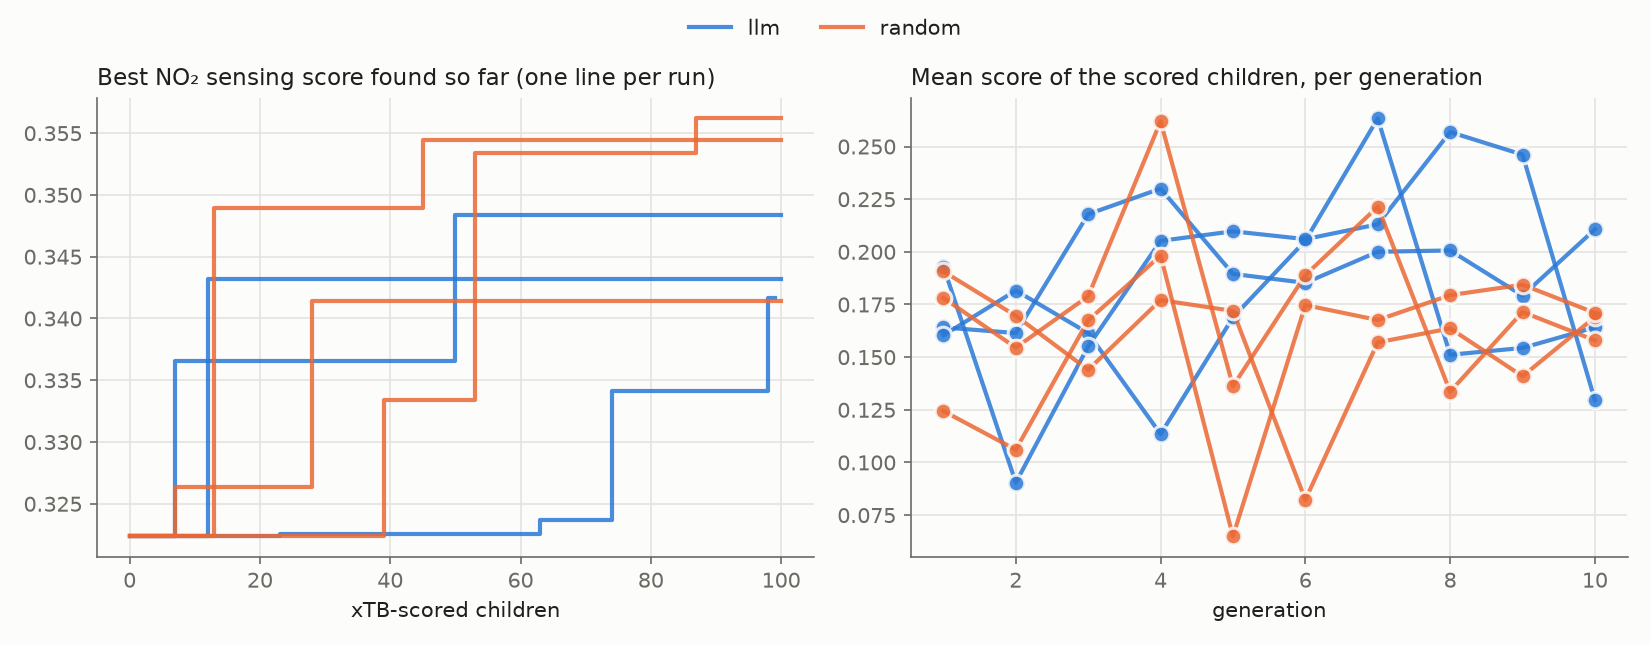
\includegraphics[width=\textwidth]{stage4_compare_v2.png}
  \caption{E5b: the six runs of loop version 2, one line per run. Left: best score found so far
           against the number of xTB-scored children (the vertical axis is zoomed in). Right: mean
           score of the scored children in each generation.}
  \label{fig:main}
\end{figure}

The changes of version 2 did what they were meant to do. Every run used the whole xTB budget (99
or 100 children, against 80 for the LLM in the pilot). Validity rose from 31\% to between 45\% and
60\% for the LLM and from 54\% to between 79\% and 84\% for random mutation, and in both cases a
large part of the valid children were open-shell proposals that the code repaired. Because more
proposals were valid, the LLM runs needed fewer of them (191 to 255, against 300 in the pilot) and
20 to 34 LLM calls per run. The full check with all gases confirmed the loop scores within 0.003
for all 30 GQDs checked. CO was the strongest competing gas for 27 of them; for the other three,
all from random runs, \ce{NH3} bound 0.001~eV more strongly than CO, which does not change their
scores.

The two mutators differ in a consistent way, but not in the way H3 predicted. Random mutation found
the best single GQD in two of the three seed pairs (0.356 and 0.354, against 0.342 and 0.343 for
the LLM), and the LLM did so in the third (0.348 against 0.341). The mean best score is 0.351 for
random mutation and 0.344 for the LLM, a difference of 0.007 that is smaller than the spread
between runs of the same mutator. On the best score, the LLM therefore shows no advantage. The mean
score of the scored children, however, was higher for the LLM in all three pairs (0.194, 0.172 and
0.191, against 0.178, 0.157 and 0.154), and its children chemisorbed \ce{NO2} less often in all
three (49 to 54\%, against 52 to 65\%). A one-sided Mann-Whitney test on the scores of all scored
children gives \(p = 0.004\) in favour of the LLM (299 against 300 children). As explained in
\cref{sec:e5}, children of one run are not independent, so this value overstates the evidence. The
number of xTB evaluations needed to pass the starting best was similar for the two mutators (23,
12 and 7 for the LLM; 39, 13 and 7 for random mutation).

In short, the LLM's proposals are better on average and avoid chemisorption somewhat more often,
while random mutation, with its larger variety of edits, found the two highest-scoring GQDs of the
study. H3 is supported for the mean score and not supported for the best score.

% ==========================================================================================
\section{E4: xTB against DFT on twelve GQDs}
\label{sec:res-e4}
% Source: Stage3a/results/dft_benchmark.md and dft_benchmark.csv (made by
% Stage3a/analyze_dft_benchmark.py from Stage3a/data/dft_benchmark/summary.csv and <gqd>/dft.csv)

All 162 single points finished and every SCF converged. \Cref{tab:e4-rho} compares the two methods
across the twelve GQDs, \cref{tab:e4-complex} compares the individual complexes, and
\cref{fig:e4-parity} shows the three quantities that make up the score.

\begin{table}[ht]
  \centering
  \caption{E4: xTB against DFT across the 12 benchmark GQDs. Each quantity is taken at the site
           and orientation where the method finds the strongest binding. The margin is the
           preference for \ce{NO2} over the strongest interfering gas.}
  \label{tab:e4-rho}
  \small
  \begin{tabular}{@{}lrrrr@{}}
    \toprule
    Quantity & Spearman \(\rho\) & Pearson \(r\) & MAE & Mean DFT \(-\) xTB \\
    \midrule
    \(E_{\ce{NO2}}\) (eV) & 0.74 & 0.87 & 0.223 & \(+0.035\) \\
    \(E_{\ce{H2O}}\) (eV) & 0.85 & 0.88 & 0.220 & \(-0.220\) \\
    \(E_{\ce{NH3}}\) (eV) & 0.95 & 0.94 & 0.144 & \(-0.144\) \\
    \(E_{\ce{CO}}\) (eV) & 0.10 & 0.12 & 0.330 & \(+0.330\) \\
    \(E_{\ce{O2}}\) (eV) & \(-0.44\) & \(-0.28\) & 1.840 & \(+1.840\) \\
    Selectivity margin (eV) & 0.86 & 0.90 & 0.269 & \(-0.167\) \\
    \(q_{\ce{NO2}}\) (\(e\)) & \(-0.11\) & \(-0.45\) & 0.185 & \(-0.185\) \\
    Sensing score (\(e\)) & \(-0.16\) & \(-0.15\) & 0.180 & \(-0.180\) \\
    \bottomrule
  \end{tabular}
\end{table}

\begin{table}[ht]
  \centering
  \caption{E4: individual complexes, grouped by the xTB geometry (bonded if the shortest contact is
           below 1.9~\AA) and by the DFT electronic state (charge-separated if more than 0.3~\(e\)
           sits on the gas). Means of adsorption energy (eV) and of the charge moved to the gas
           (\(e\)).}
  \label{tab:e4-complex}
  \small
  \begin{tabular}{@{}lllrrrrr@{}}
    \toprule
    Gas & Geometry & DFT state & \(n\) & \(\Eads\) xTB & \(\Eads\) DFT & Charge xTB & Charge DFT \\
    \midrule
    \ce{NO2} & physisorbed & neutral & 34 & \(-0.32\) & \(-0.26\) & 0.23 & 0.01 \\
    \ce{NO2} & physisorbed & charge-separated & 7 & \(-0.44\) & \(+0.52\) & 0.32 & 0.60 \\
    \ce{NO2} & bonded & neutral & 7 & \(-0.90\) & \(-0.73\) & 0.23 & 0.21 \\
    \ce{O2} & physisorbed & neutral & 12 & \(-0.69\) & \(+0.33\) & 0.39 & 0.05 \\
    \ce{O2} & bonded & both & 11 & \(-1.88\) & \(+0.88\) & 0.43 & 0.39 \\
    \ce{H2O} & physisorbed & neutral & 24 & \(-0.14\) & \(-0.32\) & 0.01 & 0.00 \\
    \ce{NH3} & physisorbed & neutral & 24 & \(-0.15\) & \(-0.26\) & 0.00 & \(-0.01\) \\
    CO & physisorbed & neutral & 24 & \(-0.21\) & \(+0.12\) & 0.07 & 0.05 \\
    \bottomrule
  \end{tabular}
\end{table}

\begin{figure}[ht]
  \centering
  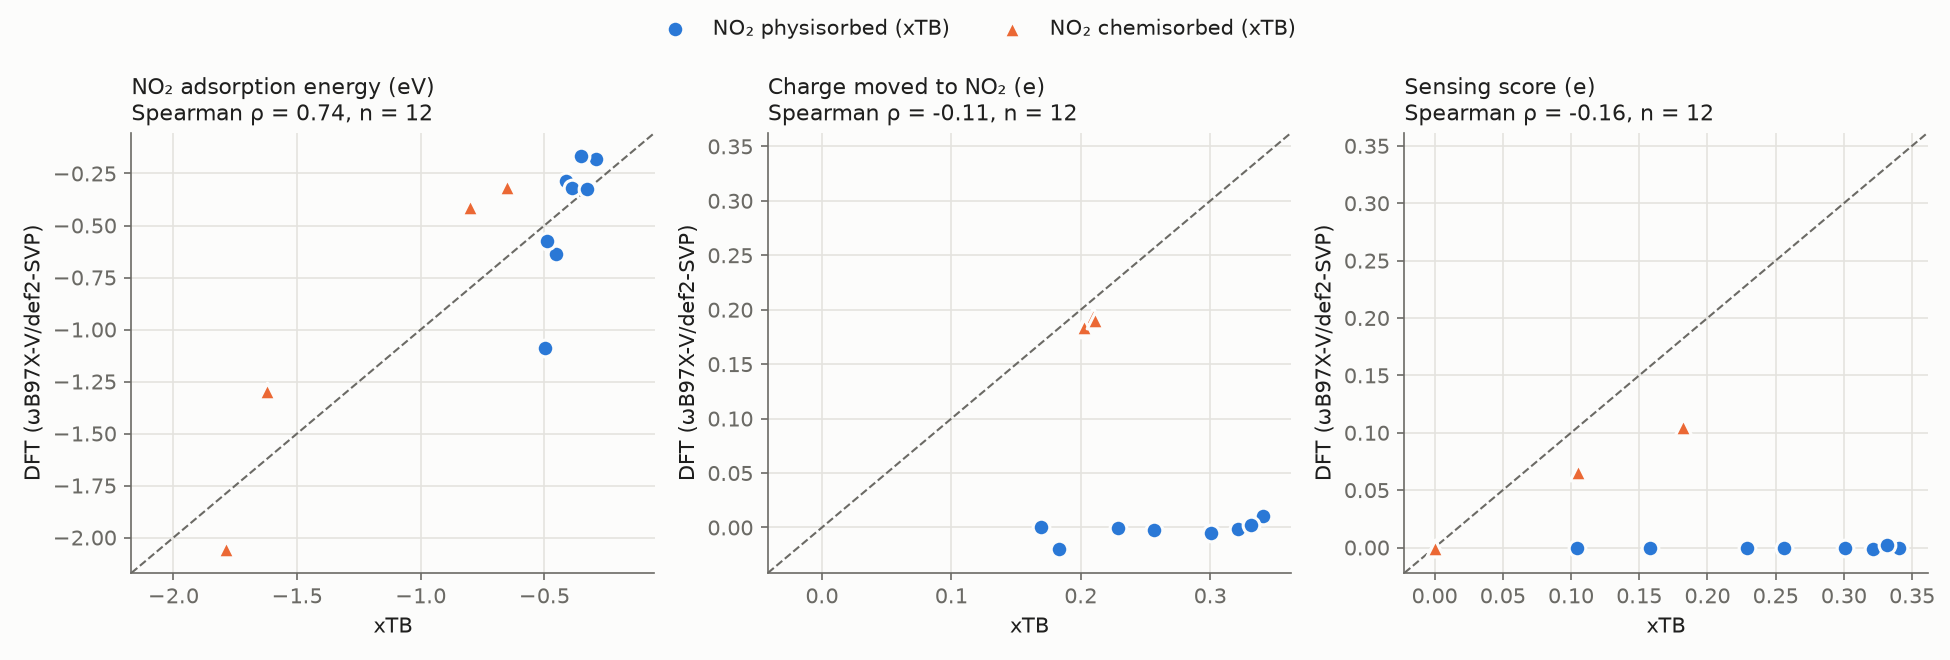
\includegraphics[width=\textwidth]{stage4_dft_vs_xtb.png}
  \caption{E4: xTB against DFT for the 12 benchmark GQDs. Left: \ce{NO2} adsorption energy.
           Middle: charge moved to \ce{NO2}. Right: sensing score. Circles: \ce{NO2} physisorbed in
           the xTB geometry; triangles: bonded. The dashed line is \(y = x\).}
  \label{fig:e4-parity}
\end{figure}

\paragraph{Binding energies are ranked well.} xTB and DFT order the GQDs in nearly the same way
for the binding of \ce{NO2} (\(\rho = 0.74\)), \ce{H2O} (\(\rho = 0.85\)) and \ce{NH3}
(\(\rho = 0.95\)), and for the selectivity margin (\(\rho = 0.86\)). For bonded \ce{NO2} the
complexes agree closely (\(\rho = 0.96\) over the seven complexes), and DFT binds them 0.18~eV less
strongly on average, consistent with the overbinding found in E3. Two systematic differences change
the selectivity picture. DFT binds \ce{H2O} and \ce{NH3} more strongly than xTB, by 0.22 and
0.14~eV on average (part of this is the basis set superposition error of def2-SVP), and it does not
bind CO at all (mean \(+0.12\)~eV). As a result, water and not CO is the strongest competing gas in
DFT for all twelve GQDs, and the selectivity margins are 0.17~eV smaller on average.

One DFT value needs care. The GQDs with the smallest gaps bind physisorbed \ce{NO2} much more
strongly in DFT than in xTB (\(-1.09\)~eV for \code{llm\_s0\_g10c004}, gap 0.29~eV, against
\(-0.50\)~eV). Small-gap GQDs may have some open-shell character in DFT. If so, the closed-shell
(RKS) energy of the bare GQD is too high, the complex (computed with UKS) can lower its energy by
spin polarisation, and the adsorption energy comes out too negative. A broken-symmetry UKS check of
the bare GQDs tested this (\cref{tab:e4-bs}). For each GQD, the RKS energy was compared with a UKS
solution started from a guess in which the HOMO and LUMO are mixed with opposite signs for the two
spins, at the same functional, basis and xTB geometry. The three GQDs with an xTB gap below 0.5~eV
have a broken-symmetry solution 0.43 to 0.82~eV below RKS, with \(\langle S^2\rangle\) of 1.5 to 1.7,
so in DFT they have strong open-shell character although each has a Kekul\'e structure. The
lowering falls as the gap grows, and \code{gqd\_88143} (gap 0.86~eV) is close to closed-shell
(0.04~eV). With the broken-symmetry energy as reference for the bare GQD, the \ce{NO2} adsorption
energy of \code{llm\_s0\_g10c004} changes from \(-1.09\) to about \(-0.27\)~eV, and
\code{random\_s0\_g02c004} no longer binds (\(+0.11\)~eV). If the UKS calculation of the complex
did not reach its own lowest broken-symmetry state, the true value lies between the two numbers.
These are single points at the xTB geometry with one functional and a small basis, and only four of
the twelve GQDs were checked. \pending{Broken-symmetry check of the other eight GQDs, including
the chemisorbing \code{gqd\_10544} (gap 0.38~eV).} This affects the energies of the small-gap GQDs,
not the charge result below: DFT also puts no charge on physisorbed \ce{NO2} for the closed-shell
\code{gqd\_88143}.

% Source: Stage3a/data/dft_benchmark/bs_check.jsonl (bs_check.py); gaps and E_NO2 DFT from
% Stage3a/data/dft_benchmark/summary.csv; also Stage3a/results/dft_benchmark.md
\begin{table}[ht]
  \centering
  \caption{E4: broken-symmetry check of the bare GQD (\(\omega\)B97X-V/def2-SVP at the xTB
           geometry). \(\Delta E\) is \(E_{\mathrm{RKS}} - E_{\mathrm{BS\text{-}UKS}}\). The last
           column is the DFT \ce{NO2} adsorption energy with the broken-symmetry energy of the GQD
           as reference.}
  \label{tab:e4-bs}
  \begin{tabular}{lrrrrr}
    \toprule
    GQD & xTB gap (eV) & \(\Delta E\) (eV) & \(\langle S^2\rangle\) & \(\Eads\) RKS ref.\ (eV)
        & \(\Eads\) BS ref.\ (eV) \\
    \midrule
    \code{llm\_s0\_g10c004}    & 0.29 & 0.82 & 1.67 & \(-1.09\) & \(-0.27\) \\
    \code{random\_s0\_g02c004} & 0.36 & 0.68 & 1.48 & \(-0.58\) & \(+0.11\) \\
    \code{gqd\_18941}          & 0.49 & 0.43 & 1.67 & \(-0.64\) & \(-0.20\) \\
    \code{gqd\_88143}          & 0.86 & 0.04 & 0.62 & \(-0.17\) & \(-0.13\) \\
    \bottomrule
  \end{tabular}
\end{table}

\paragraph{Charge transfer to physisorbed \NOtwo{} is an xTB artefact.} This is the main result of
the benchmark. In the 34 physisorbed complexes in the lowest DFT state, the charge on \ce{NO2} is
0.01~\(e\) on average, against 0.23~\(e\) in xTB at the same geometries. DFT places the unpaired
electron on \ce{NO2} and leaves the GQD neutral. A charge-transfer state does exist: in seven
complexes the DFT calculation converged to a state with about 0.6~\(e\) on \ce{NO2}, but this
state lies above the separated molecules (mean \(\Eads = +0.52\)~eV) and is therefore not the
state of the adsorbed molecule. For bonded \ce{NO2}, the two methods agree on the charge (0.23
and 0.21~\(e\)). The small-model check of E3 already showed this effect on coronene; the
benchmark shows that it holds for every physisorbing GQD.

\paragraph{The score does not survive.} Because the response term of the score is the charge moved
to \ce{NO2}, the DFT score of every physisorbing GQD is close to zero (\(|S| \leq 0.002\)), including
the best GQDs of both pilot runs (0.000 and 0.002, against 0.341 and 0.331 in xTB). The rank
correlation of the score is \(\rho = -0.16\), and among the eight physisorbing GQDs it is 0.08. By
the rule fixed in \cref{sec:e4} (\(\rho < 0.4\)), \emph{the score must change}. Only two GQDs keep
a non-zero DFT score, \code{gqd\_13400} (0.105) and \code{gqd\_58903} (0.066). Both bond to
\ce{NO2} in xTB, and in DFT this bond is weak enough to be reversible (\(-0.31\) and
\(-0.41\)~eV) while it still moves about 0.19~\(e\) to \ce{NO2}. At the level of DFT, a weak
covalent bond, and not physisorption, is what combines a clear response with recovery.

\paragraph{\ce{O2} does not bind.} xTB binds \ce{O2} by \(-0.76\) to \(-2.82\)~eV, while DFT finds
\ce{O2} unbound on eleven of the twelve GQDs (adsorption energies up to \(+0.99\)~eV), including
both pilot bests (\(+0.41\) and \(+0.55\)~eV). The exception, \code{gqd\_18941}, physisorbs \ce{O2}
weakly (\(-0.20\)~eV). At this level of theory, none of the benchmark GQDs is at risk of
binding oxygen from air, and the large xTB \ce{O2} energies are again an artefact. These are single
points at xTB geometries, so a DFT optimisation of a bonded \ce{O2} complex could still find a
bound minimum that the xTB geometry misses.

% ==========================================================================================
\section{Features of the best GQDs}
\label{sec:res-best}
% Source: final_check.csv of llm_s0, random_s0 and the six v2 runs (40 GQDs)

Across the 40 best GQDs that received the full check (five from each of the eight runs), a
consistent pattern appears. All of them physisorb \ce{NO2}. They have 29 to 40 hexagons and xTB
gaps of 0.23 to 0.57~eV, and the ten highest-scoring ones have gaps of 0.26 to 0.43~eV. \ce{NO2}
binds at \(-0.43\) to \(-0.52\)~eV, takes 0.311 to 0.356~\(e\), and is preferred over the strongest
competing gas by 0.16 to 0.28~eV and over \ce{H2O} by 0.25 to 0.36~eV.

Because every one of these GQDs binds \ce{NO2} more weakly than \(-0.6\)~eV and prefers it over
the competing gases by more than 0.10~eV, both factors of the score equal 1 for all 40, and the
score is simply the xTB charge moved to \ce{NO2}. Among the best GQDs, the ranking therefore rests
entirely on the physisorbed charge, the quantity that xTB overestimates
(\cref{sec:res-dft-small}). This makes the DFT benchmark of \cref{sec:res-e4} the deciding test for
these candidates.

Compared with the best calibration GQDs (gaps of 0.49 to 0.67~eV), the loops therefore moved toward
smaller gaps while keeping \ce{NO2} physisorbed at the two probed sites. This is the region that
\cref{sec:res-e2} identified as most promising and most difficult, since most dataset GQDs with
small gaps chemisorb \ce{NO2}.
\pending{Structural analysis of the best GQDs (edge types, Clar sextets, position of the binding
site) and a figure of their shapes.}

% Chapter 6. Revisit each research question when its experiment finishes; keep the
% limitations section honest and specific.
\chapter{Discussion}
\label{ch:discussion}

\section{RQ1: can the LLM design valid GQDs in hexagon coordinates?}

Yes, provided that the code explains its rejections in terms the LLM can act on. Writing hexagon
positions removed the problems that make long SMILES strings hard to write: the LLM produced
connected lists of roughly the requested size, and almost all of its valid designs were new. What
it could not do was see whether a shape is closed-shell. This is a global property of the whole
structure. A shape that looks reasonable can have one more atom on one sublattice than on the
other, and nothing in a single coordinate pair reveals it. In the first run, 66 of 67 failed
attempts were open-shell.

The two aids address this in different ways. The rule in the prompt gives the LLM a way to avoid
the problem, mainly by building point-symmetric shapes, and it raised the first-attempt pass rate.
The fix edits turn the global condition into a short list of local actions, and they made retries
succeed. Together they reached 99\%, which supports H1. The price is less variety, because the
rule pushes the LLM toward a few safe symmetric shapes. For the agent, which rejects repeats, this
price is acceptable, and the evolutionary loop gets its variety from the parents it edits.

The loop showed that validity is not settled by the representation alone. When the LLM edited
existing GQDs rather than designing new ones, other errors appeared: adding a hexagon that was
already present, removing one that was not, proposing a duplicate, or using more edits than
allowed. The repair step in version 2 recovered many of these children. The general lesson is to
divide the work by what each side can check. The LLM works in a representation where a small
change to the shape is a small change to the text, and the code handles global constraints and
returns actionable feedback.

\section{RQ2: can xTB rank GQDs for \NOtwo{} sensing?}

The small-model check (E3) answers part of this question. For physisorption, which is the regime
of every top candidate, xTB adsorption energies are close to DFT. For chemisorption, xTB is
qualitatively right but overbinds by 0.1 to 0.55~eV, and the reversibility window of the score was
placed with this error in mind. For \ce{O2}, xTB is wrong: it binds a molecule that DFT does not
bind at all. The charge transferred to physisorbed \ce{NO2} is too large in xTB, but it follows the
HOMO energy of the GQD (\(r = 0.88\)), which is the right physical trend.

The results of the loop sharpened this question. For all 40 best GQDs, the reversibility and
selectivity factors equal 1, so the score of the best candidates is the xTB charge alone
(\cref{sec:res-best}). The ranking at the top therefore depended on the one quantity that xTB was
suspected to overestimate.

The GPU benchmark (E4) answers the question, and the answer is split. xTB ranks GQDs well by how
strongly they bind \ce{NO2}, \ce{H2O} and \ce{NH3} (\(\rho = 0.74\) to 0.95) and by their
selectivity margin (\(\rho = 0.86\)), so for binding and selectivity H2 is supported. It does not
rank them by charge transfer (\(\rho = -0.11\)), because in DFT physisorbed \ce{NO2} takes almost
no charge at all (0.01~\(e\) against 0.23~\(e\) in xTB). H2 is therefore contradicted for the
response, and with it for the score (\(\rho = -0.16\)). By the rule fixed in advance, the score has
to change. Two further corrections follow from DFT: water, not CO, is the most dangerous
competing gas, and \ce{O2} does not bind, so the air-stability concern raised by the xTB \ce{O2}
energies disappears at this level of theory.

The consequences for the earlier results are direct. The best GQDs of both the calibration and
the evolutionary loops were selected for a large xTB charge on physisorbed \ce{NO2}, and in DFT
this charge is close to zero. They remain GQDs that bind \ce{NO2} selectively and reversibly, but
they are not shown to give a large electronic response. What the loops optimised was, in effect,
an xTB artefact that follows the HOMO energy. The comparison of the mutators (RQ3) is not affected
as a test of search methods, because both mutators optimised the same objective, but its winners
are not validated sensor candidates.

The broken-symmetry check adds a second problem for the same GQDs (\cref{tab:e4-bs}). The GQDs
with the smallest xTB gaps, which include the best GQDs of both pilot runs, have strong open-shell
character in DFT (\(\langle S^2\rangle \approx 1.5\) to 1.7 and a lowering of up to 0.82~eV), even
though each has a Kekul\'e structure. The closed-shell rule of the pipeline is a test of the
graph, and it does not exclude this. Both the closed-shell xTB scores and the RKS-referenced DFT
energies of these GQDs therefore rest on a reference state that is not the lowest one, and the
strong DFT binding of \ce{NO2} on them is mostly an artefact of that reference. The charge result
does not depend on this, since the nearly closed-shell \code{gqd\_88143} also shows no charge on
\ce{NO2}. The check covers four GQDs with one functional at xTB geometries, so it shows that the
problem exists but not where the gap limit lies. How to treat open-shell character is open
(\code{RESEARCH\_OPTIONS.md}, D22).

Three ways to repair the score are open (\code{RESEARCH\_OPTIONS.md}, D7). The response could be
taken from DFT for the final candidates only, which is accurate but too slow for the loop. It could
be replaced by an orbital descriptor, such as the alignment of the GQD's HOMO with the singly
occupied orbital of \ce{NO2}, which can be computed cheaply and has a clear physical meaning. Or the
target could move to the regime that DFT favours: a weak, reversible covalent bond to \ce{NO2}
(about \(-0.3\) to \(-0.6\)~eV), which in DFT still moves about 0.2~\(e\). The two benchmark GQDs
that keep a non-zero DFT score are of this kind. Separately, the sensor model proposed in
\cref{sec:future} would help with all three, because a real chemiresistor responds to the change
in carrier density of the film, and that depends on more than the net charge on one molecule.

\section{RQ3: does the LLM find better GQDs than random mutation?}

The answer depends on what is measured. With three runs per mutator, the LLM's children scored
higher on average in every pair of runs (0.186 against 0.163 over all runs) and chemisorbed
\ce{NO2} less often, so its edits are better than random ones on average. But the best GQD came
from random mutation in two of the three pairs, and the mean best score was 0.351 for random
mutation against 0.344 for the LLM. For the goal of the search, which is the best GQD found within
the budget, the LLM gave no advantage. H3 is supported for the mean score and not supported for the
best score. The pilot, in which the LLM found the best GQD, was within this run-to-run variation.
Several reasons can explain this outcome.

First, the headroom is small. The best starting GQD scored 0.322 and the best GQD found so far
scores 0.356, a gain of about 10\%. Gains of a few hundredths are close to the noise of the score,
which comes from xTB itself and from probing only two adsorption sites. Second, the score
saturates. Once a GQD physisorbs \ce{NO2} with a good margin over CO, the score equals the charge
transfer, and the remaining differences are small changes in a single number. Third, random edits
with automatic repair are a strong local search on this problem. Most single-hexagon edits produce
a valid, similar GQD, and the population keeps the good ones. The MolLEO study reports a similar
observation for drug-like molecules: in some settings the default graph-based mutation performed
about as well as LLM mutation while using fewer LLM queries \cite{wang2024molleo}.
\authornote{Check this statement against the MolLEO paper before submission.} Fourth, the LLM was asked to make
mostly refinements of the best parents, which favours exploitation over exploration. Careful
refinements raise the average, while the best GQD of a run is an outlier, and the wider variety of
random edits produces more outliers. The pilot also showed that the LLM's multi-edit proposals fail
more often than single edits.

The LLM run has value beyond the best score. Every LLM edit comes with a stated reason, which makes
its choices auditable, and the logged reasons and outcomes are the material for fine-tuning a model
that may propose better edits than either mutator. Three runs per mutator are few, so these conclusions should be
checked with more runs. \pending{Comparison with the baseline without evolution (E6).}

\section{RQ4: what do the best GQDs have in common?}

The calibration (E2) showed the trade-off of H4: a smaller gap raises the charge given to \ce{NO2},
but most small-gap GQDs chemisorb it and lose the ability to recover. The best calibration GQDs
balanced the two at gaps of 0.49 to 0.67~eV. Both loops then found GQDs with smaller gaps, 0.26 to
0.43~eV for the ten best, that still physisorb \ce{NO2} at both probed sites, and these scored
higher. All of the best GQDs have 29 to 40 hexagons, bind \ce{NO2} at about \(-0.43\) to
\(-0.52\)~eV and prefer it over the strongest competing gas by at least 0.16~eV. These results support H4 at the xTB level.

DFT changes this picture (E4). The first half of the trade-off, a larger response at a smaller gap,
rests on the physisorbed xTB charge, which DFT does not reproduce. In DFT, the response survives
only where \ce{NO2} forms a bond, and the two benchmark GQDs with a non-zero DFT score form a weak
one (\(-0.31\) and \(-0.41\)~eV). The design target that DFT suggests is therefore a weak,
reversible bond to \ce{NO2} rather than physisorption, so H4 is not supported at the DFT level.

Two further cautions apply. Chemisorption depends on the local site, and only two sites were
probed, so a GQD that physisorbs \ce{NO2} at its centre and its most exposed edge may still
chemisorb it elsewhere. Small-gap GQDs are generally more reactive, but in DFT \ce{O2} did not bind
eleven of the twelve benchmark GQDs, including both pilot bests, so air stability is not a concern
at this level of theory.

\section{Limitations}
\label{sec:limitations}

\paragraph{Model of the sensor.} Every calculation describes one gas molecule on one isolated GQD
in the gas phase at 0~K. The model leaves out the substrate, the electrical contacts, the
coverage of gas molecules, humidity, temperature and the arrangement of GQDs in a real film. The
response is represented by the charge moved to \ce{NO2}, which is a proxy for the change in
conductance and not a prediction of it. Recovery is estimated from the adsorption energy alone.

\paragraph{Sites and configurations.} Only two adsorption sites are probed, and each interfering
gas is tried in one orientation. Optimisations start from one height and can end in a local
minimum. For final candidates, all symmetry-distinct sites should be checked.

\paragraph{Level of theory.} The score is computed with xTB, whose weaknesses for charge transfer
and \ce{O2} are documented above. The DFT checks are single points at xTB geometries with a small
basis set and no counterpoise correction, and atomic charges depend on the partitioning scheme.

\paragraph{Chemical space.} Only pure-carbon, closed-shell GQDs with 20 to 40 hexagons and no holes
are considered, and shapes whose SMILES RDKit cannot re-read are excluded. ``New'' means absent from
our dataset of 91{,}174 structures, not absent from the literature.

\paragraph{The LLM.} The LLM is a commercial model accessed through an API. Its replies cannot be
seeded, and the model behind a deployment may change over time. The logged prompts and replies make
every run auditable, but an LLM run cannot be repeated exactly. LLM calls are not counted in the xTB
budget, and their cost and time were not measured.

\paragraph{Statistics and design choices.} Three runs per mutator give limited statistical power
(\cref{sec:e5}), and children within a run are not independent. Several settings of the loop, such
as the gap window, the family cap, the amount of history shown to the LLM and the strategy hint in
the prompt, were chosen once and not tuned for either mutator. A different choice could favour one
of them.

\paragraph{Predictor.} The gap predictor is trained on the dataset distribution and is used only as
a filter. Its window can remove good children, as the pilot's 0.30~eV floor did.

\section{Practical cost}

One full xTB evaluation takes about a minute on the laptop, and inside the loop ten children are
scored in about 3 to 6 minutes, so a ten-generation run takes about an hour. A run used 27 to 34
LLM calls. The DFT benchmark of 12 GQDs needs 162 single points, about 12 hours on one A100, or
roughly one hour per GQD with all gases. The work was split by hardware: the xTB loop ran on the
laptop CPU, which was six times faster for xTB than the shared server CPU, and DFT ran on the
server GPU. This split kept each kind of calculation on the hardware that suits it.

% Chapter 7. Update the summary when a research question gets its final answer, and move
% items from future work into the main text when they are done.
\chapter{Conclusion and future work}
\label{ch:conclusion}

\section{Conclusion}

This thesis built an agent workflow for designing graphene quantum dots for \ce{NO2} sensing, in
which an LLM proposes structures and code and quantum chemistry decide which ones are valid and
good. The LLM writes GQDs as hexagon positions on a honeycomb grid. Code converts them into
molecules exactly, checks the closed-shell condition with a matching algorithm, and explains every
rejection with edits that would fix it. With this feedback and the closed-shell rule in the prompt,
99\% of design requests ended in a valid GQD, against 52\% without them (RQ1).

An \ce{NO2} sensing score was defined from GFN2-xTB calculations of adsorption energy and charge
transfer for \ce{NO2} and the competing gases. On 50 dataset GQDs it identified a design target that
was not chosen by hand: a moderately small gap together with physisorption of \ce{NO2}. A DFT check
showed that xTB is reliable for physisorption energies, overbinds chemisorbed \ce{NO2}, inflates
the physisorbed charge and fails for \ce{O2} (RQ2, in part).

In an evolutionary loop with the same xTB budget, both the LLM and random mutation improved on the
best starting GQD: its score was 0.322, and the eight runs reached best scores of 0.331 to 0.356.
Both moved toward GQDs with gaps of about 0.3 to 0.4~eV that still physisorb \ce{NO2} (RQ4). With
three runs per mutator, the LLM's children scored higher on average in every pair of runs, but
random mutation found the best GQD in two of the three pairs, so the LLM did not find better GQDs
than random mutation (RQ3).

Among the best GQDs the score reduces to the xTB charge transfer, and the DFT benchmark of twelve
GQDs showed that this charge is an artefact: in DFT, physisorbed \ce{NO2} takes almost no charge
(0.01~\(e\) against 0.23~\(e\)), and the score loses its ranking (\(\rho = -0.16\)). xTB remains
useful for what it ranks well, the binding of \ce{NO2}, \ce{H2O} and \ce{NH3} and the selectivity
margin (\(\rho = 0.74\) to 0.95), and DFT removes the \ce{O2} concern, since \ce{O2} does not bind
(RQ2). The workflow therefore works as a search method, but the objective it searched needs a new
response term before its best GQDs can be called good sensors. In DFT, the GQDs that keep a
response are those that form a weak, reversible bond to \ce{NO2}.
\pending{The baseline without evolution (E6).}

\section{Future work}
\label{sec:future}

\paragraph{Replace the response term.} The DFT benchmark shows that the xTB charge on physisorbed
\ce{NO2} cannot serve as the response. The candidates are an orbital descriptor such as the
alignment of the GQD's HOMO with the singly occupied orbital of \ce{NO2}, a correction learned from
DFT data, or a new target regime of weak, reversible chemisorption, which in DFT keeps a clear
charge transfer. The selectivity term should use water as the main competitor. The loops should
then be repeated with the new score, and the best candidates re-ranked with DFT.

\paragraph{A sensor model.} A model of the sensing film, with gas coverage at real concentrations
and humidity, adsorption and desorption kinetics, and the resulting change in resistance, would
turn the molecular numbers into a predicted sensor signal and give the search a device-level goal.

\paragraph{Complete the current experiments.} Add the baseline without evolution (E6) and repeat
the comparison of E5b with more runs per mutator.

\paragraph{Check the final candidates more thoroughly.} Probe all symmetry-distinct adsorption
sites and optimise the most promising complexes, including any bonded \ce{O2} complex, at the DFT
level instead of using xTB geometries.

\paragraph{Beyond pure carbon (Stage 3b).} Nitrogen and boron dopants and edge groups such as
\ce{-OH}, \ce{-COOH} and \ce{-NH2} change how strongly gases bind \cite{zhang2009dopants} and may
offer much more headroom than shape alone. This needs a representation that labels individual
atoms, new validity rules (dopants change the electron count and therefore the closed-shell
condition), a new gap predictor or none, and a recalibrated score.

\paragraph{A surrogate for the sensing score.} The logs of the loop contain hundreds of xTB-scored
GQDs with all their descriptors. A model trained on them could replace part of the xTB budget, in
the same way that the gap predictor does for the gap.

\paragraph{Fine-tuning a smaller model.} The logs are designed to become three training sets: edits
that improved the score (supervised fine-tuning), pairs of better and worse edits of the same
parent (preference training with DPO \cite{rafailov2023dpo}), and target-to-structure examples from
the 14{,}674 labelled dataset GQDs and the scored children. A small open model of about 7 to 8
billion parameters, fine-tuned with LoRA \cite{hu2022lora}, could then be tested in the same loop
against random mutation and the general-purpose LLM.

\paragraph{Generative models as further baselines.} Models trained on SELFIES strings
\cite{krenn2020selfies}, graph or diffusion models that work directly on the hexagon grid, and
reinforcement learning in the style of REINVENT \cite{olivecrona2017reinvent} would place the
LLM-guided loop among established methods.


% ------------------------------------------------------------------ appendices
\appendix
\crefalias{chapter}{appendix}
% Appendix A. Prompts are copied verbatim from the code and run logs; update them if the
% prompts in studio/agent.py or Stage3/evolve.py change.
\chapter{LLM prompts}
\label{app:prompts}

The prompts are reproduced exactly as they were sent, including their wording errors. Values that
the code inserts (size limits and score thresholds) are shown as they were filled in.

\section{System prompt of the agent}

From \code{studio/agent.py}. The part from ``Hexagon rules'' to ``lists edits that fix it'' is the
closed-shell rule tested in E1 (the \emph{rule} prompt); the \emph{basic} prompt of E1 contained
only the coordinate, neighbour and size rules.

\begin{lstlisting}
You are a helpful assistant tasked with generate GQD, validate software and environment. To design a GQD yourself, call build_gqd_from_hexagons with hexagon coordinates (never write SMILES). Hexagon rules: each hexagon is [q, r] in axial coordinates; the six neighbours of [q, r] are [q+1, r], [q-1, r], [q, r+1], [q, r-1], [q+1, r-1], [q-1, r+1]. All hexagons must form one connected piece, with no duplicates, 20-40 hexagons. The GQD must be closed-shell: its carbon atoms form two alternating sets (sublattices) that must be equal in number. Triangular shapes, L-shaped corners and long zigzag edges usually break this and are rejected as open-shell. A reliable way to stay closed-shell is a point-symmetric shape: pick a centre and, for every [q, r] in the list, also include [a-q, b-r] (for example with a = b = 0, [2, -1] needs [-2, 1]). If a requested shape cannot be closed-shell, build the closest closed-shell variant. If a design is rejected, the message explains why and lists edits that fix it. Call one tool at a time. If a design you made is rejected, fix it yourself using the rejection message (for example apply one of the suggested edits) and call the tool again, without asking the user; give up after 3 rejected attempts for the same request and report why. Each generated GQD is validated automatically and then accepted or rejected. Once a GQD is accepted, report it to the user; only design another new GQD if the user asked for more.
\end{lstlisting}

\section{System prompt of the LLM mutator}

From \code{Stage3/results/llm\_v2\_s1/config.json} (loop version 2).

\begin{lstlisting}
You improve graphene quantum dots (GQDs) for an NO2 gas sensor. A GQD is a set of fused hexagons on a honeycomb grid, written as [q, r] positions. Hexagon rules: each hexagon is [q, r] in axial coordinates; the six neighbours of [q, r] are [q+1, r], [q-1, r], [q, r+1], [q, r-1], [q+1, r-1], [q-1, r+1]. All hexagons must form one connected piece, with no duplicates, 20-40 hexagons. The GQD must be closed-shell: its carbon atoms form two alternating sets (sublattices) that must be equal in number. Triangular shapes, L-shaped corners and long zigzag edges usually break this and are rejected as open-shell. A reliable way to stay closed-shell is a point-symmetric shape: pick a centre and, for every [q, r] in the list, also include [a-q, b-r] (for example with a = b = 0, [2, -1] needs [-2, 1]). If a requested shape cannot be closed-shell, build the closest closed-shell variant. If a design is rejected, the message explains why and lists edits that fix it. How a GQD is scored (xTB calculations; higher is better): sensing score = charge moved to NO2 (e) x reversibility x selectivity. Reversibility is 1 if NO2 binds no more strongly than -0.6 eV (so it can leave again) and falls to 0 at -1.0 eV (NO2 forms a chemical bond and stays). Selectivity is 1 if NO2 binds at least 0.1 eV more strongly than CO, the strongest competing gas. NO2 is tested above two hexagons of each GQD: the most central one and the most exposed edge one. You make children by editing a parent: ADD [q, r] puts a new hexagon next to the shape, REMOVE [q, r] takes one away (the rest must stay connected). Each child is 1-3 edits on one parent. A child must be a new structure (not made before in this run and not in our 91k-structure dataset), closed-shell, 20-40 hexagons, without holes. If a child is open-shell, code first tries to repair it by adding or removing one hexagon (shown in the results as 'code added ...'). If a child is still rejected, any fix edits in the message apply to the child, so append one to that child's edits. Study how the high-scoring GQDs differ from the low-scoring ones, then propose edits you expect to raise the score: mostly refinements of the best parents, plus a few bolder changes.
\end{lstlisting}

\section{Example exchange}

An excerpt of the user message in generation 5 of run \code{llm\_v2\_s1}, followed by the first
three children of the LLM's reply (from \code{llm\_log.jsonl}). Long lines are shortened with
``\ldots''.

\begin{lstlisting}
Generation 5. Goal: maximise the NO2 sensing score (charge to NO2 x reversibility x selectivity vs CO).

Current population (best first):
g03c005 | score 0.323 | 34 hexagons | gap 0.44 eV | NO2 -0.46 eV, physisorbed, best at the edge hexagon [0, 0], charge 0.32 e | NO2 vs CO margin +0.19 eV
  hexagons: [[-5,2],[-4,-2],[-4,-1],[-4,0],[-4,1],[-4,2], ... ,[0,0],[-4,5],[-5,-1]]
gqd_18941 | score 0.322 | 30 hexagons | gap 0.49 eV | NO2 -0.45 eV, physisorbed, best at the centre hexagon [-3, 3], charge 0.32 e | NO2 vs CO margin +0.20 eV
...
Last generation's children (parent -> edits -> result):
- g02c004 -> REMOVE [-5, 0]; REMOVE [-5, 3]; ADD [-5, -1] -> not scored: duplicate: this structure was already made in this run
- g03c005 -> REMOVE [-5, 2]; REMOVE [-5, -1] -> not scored: molecular graph: structure has no Kekulé form (open-shell / radical GQD): its carbon atoms form two alternating sets (sublattices) that must be equal in size, but here they are 53 vs 51 (2 unpaired atom(s); ...
- g03c005 -> REMOVE [-4, 8]; REMOVE [-4, -2] (code added ADD [-5, 4] to make it closed-shell) -> score 0.121 (parent 0.323); NO2 -0.76 eV chemisorbed, gap 1.28 eV, charge 0.20 e
- g03c005 -> REMOVE [-4, 6]; REMOVE [-2, -2] -> score 0.255 (parent 0.323); NO2 -0.38 eV physisorbed, gap 0.50 eV, charge 0.25 e
...
\end{lstlisting}

\begin{lstlisting}
{"parent_id": "g03c005", "edits": [{"op": "ADD", "q": -5, "r": 1}, {"op": "REMOVE", "q": -5, "r": 2}], "reason": "Shifts one exposed edge notch downward while keeping size and connectivity, aiming to preserve the strong edge NO2 site but slightly increase charge transfer without overbinding."}
{"parent_id": "g03c005", "edits": [{"op": "ADD", "q": -5, "r": 3}, {"op": "REMOVE", "q": -5, "r": 2}], "reason": "Moves the lone outer-left protrusion closer to the upper active edge to tune the local electrostatics and possibly strengthen NO2 binding only modestly."}
{"parent_id": "g03c005", "edits": [{"op": "ADD", "q": -5, "r": 4}, {"op": "REMOVE", "q": -4, "r": 8}], "reason": "Trims the most remote upper tip while filling a nearby indentation, which should reduce excessive edge irregularity and retain a high-charge exposed adsorption site."}
\end{lstlisting}

% Appendix B. Keep in line with the record written by Stage3/evolve.py (run_generation).
\chapter{Logged fields of the evolutionary loop}
\label{app:logging}

Each line of \code{Stage3/results/<run>/children.jsonl} describes one proposed child, including
rejected and skipped ones. The first group contains the fields required for the fine-tuning
datasets; the others record the details needed to reproduce and analyse a run.

\begin{table}[ht]
  \centering
  \caption{Fields of one child record.}
  \label{tab:fields}
  \small
  \begin{tabularx}{\textwidth}{@{}lL@{}}
    \toprule
    Field & Meaning \\
    \midrule
    \multicolumn{2}{@{}l}{\emph{Required for the fine-tuning datasets}} \\
    \code{generation} & generation number (1 to 10) \\
    \code{goal} & the objective in words (maximise the \ce{NO2} sensing score) \\
    \code{parent\_id}, \code{parent\_hexagons}, \code{parent\_score} & the parent and its score \\
    \code{edit} & the edits, for example \code{ADD [-5, 1]; REMOVE [-5, 2]} \\
    \code{reason} & the LLM's one-sentence reason (``random edit'' for the random mutator) \\
    \code{child\_hexagons} & the child's hexagon list (after any repair) \\
    \code{valid}, \code{reject\_reason} & whether the child passed all checks, and why not \\
    \code{predicted\_gap} & gap predicted by the Stage 2 model (eV) \\
    \code{xtb\_gap} & xTB gap of the optimised child (eV), if scored \\
    \midrule
    \multicolumn{2}{@{}l}{\emph{Loop bookkeeping}} \\
    \code{run}, \code{mutator}, \code{child\_id}, \code{round} & run name, mutator, identifier, proposal round \\
    \code{smiles}, \code{n\_hex} & canonical SMILES and number of hexagons \\
    \code{repair} & the edit added by code to make an open-shell child closed-shell \\
    \code{root} & the starting GQD of the child's family \\
    \code{predicted\_gap\_sigma} & uncertainty of the predicted gap (eV) \\
    \code{skip\_reason} & why a valid child was not scored (gap window or budget) \\
    \code{evaluated} & whether the child was scored with xTB \\
    \midrule
    \multicolumn{2}{@{}l}{\emph{xTB results (scored children)}} \\
    \code{E\_NO2\_eV}, \code{q\_NO2\_e}, \code{dmin\_NO2\_A} & \ce{NO2} adsorption energy, charge and shortest contact \\
    \code{NO2\_chemisorbed}, \code{NO2\_site}, \code{NO2\_site\_cell} & bonded or not, and where \ce{NO2} binds best \\
    \code{E\_CO\_eV}, \code{selectivity\_margin\_eV} & CO adsorption energy and the margin of \ce{NO2} over CO \\
    \code{reversibility}, \code{charge\_to\_NO2\_e}, \code{sensing\_score} & the factors and the score \\
    \code{all\_converged}, \code{xtb\_details}, \code{xtb\_seconds} & convergence, per-job results, run time \\
    \bottomrule
  \end{tabularx}
\end{table}

Each run folder also contains these files:
\begin{itemize}
  \item \code{config.json}: the settings and the system prompt;
  \item \code{generations.jsonl}: one summary line per generation;
  \item \code{llm\_log.jsonl}: every prompt and reply of the LLM mutator;
  \item \code{summary.md}: a readable summary of the run;
  \item \code{final\_check.csv}: the full check of the five best new GQDs.
\end{itemize}

% Appendix C. Add the command for every new experiment.
\chapter{Reproducing the results}
\label{app:reproduce}

All code is in the \code{Agentic\_GQD} folder of the project repository, one folder per stage, each
with a README. Commands are run from \code{Agentic\_GQD} with the project's Python environment
(\code{.venv}). The LLM steps need Azure OpenAI settings in \code{studio/.env}, which are not part of
the repository. xTB runs use the conda-forge build of xTB 6.7.1; the path can be set with the
\code{XTB\_BIN} environment variable.

\begin{table}[ht]
  \centering
  \caption{Commands for each stage.}
  \label{tab:commands}
  \small
  \begin{tabularx}{\textwidth}{@{}lL@{}}
    \toprule
    Stage & Command and notes \\
    \midrule
    1  & \code{.venv/bin/python Stage1/build\_hex\_dataset.py} (about 3 minutes) \\
    2  & \code{.venv/bin/python Stage2/build\_features.py}, then
         \code{.venv/bin/python Stage2/train.py --trials 100 --folds 5 --gnn-epochs 300}
         (about 80 minutes on the laptop CPU) \\
    2d & \code{.venv/bin/python Stage2d/llm\_hexagon\_test.py --n 80 --retries 2}
         (about 550 LLM calls, about 10 minutes) \\
    3a & \code{.venv/bin/python Stage3a/calibrate.py --n 50}, then
         \code{.venv/bin/python Stage3a/analyze.py}; small-model DFT with
         \code{Stage3a/dft\_check.py} and \code{Stage3a/xtb\_vs\_dft.py} \\
    3, 4 & \code{.venv/bin/python Stage3/evolve.py --run llm\_v2\_s1 --mutator llm --seed 1
         --generations 10 --children 10 --parallel 5} (and \code{--mutator random}; seeds 1 to 3);
         then \code{.venv/bin/python Stage3/compare.py <runs> --name v2} \\
    DFT & \code{Stage3a/make\_geometries.py} writes the geometries; on the GPU server,
         \code{CUDA\_VISIBLE\_DEVICES=0 python Stage3a/dft\_gpu.py Stage3a/data/dft\_benchmark};
         environments from \code{server/setup\_envs.sh} \\
    \bottomrule
  \end{tabularx}
\end{table}

A run of \code{evolve.py} that stops can be restarted with the same \code{--run} name, and it
continues after the last finished generation. \code{dft\_gpu.py} keeps every finished calculation
in \code{dft\_results.jsonl} and also resumes where it stopped; \code{--summary-only} writes the
comparison tables from the finished calculations.


% ------------------------------------------------------------------ references
\cleardoublepage
\phantomsection
\addcontentsline{toc}{chapter}{References}
\bibliographystyle{unsrtnat}
\bibliography{references}

\end{document}
